\chapter{Fluxonium in a 3D Cavity: Experiments\label{ch:4_3DGKP}}
In this chapter, we will introduce our first experimental implementation using fluxonium as the control qubit for an oscillator. In this experiment, we integrated a heavy fluxonium chip into a 3D superconducting cavity resonator architecture. We will start by introducing the basic idea behind the experiment in Sec. \ref{sec:4_3D_Experiment_Design_Theory}, followed by a discussion of the hardware we used to implement it in \ref{sec:4_Hardware_and_Setup}. We will then present an assortment of experimental results that we obtained with this system in Secs. \ref{sec:4_Resonator_and_Two_Tone}-\ref{sec:4_StorageCoherenceProblems}, highlighting both our successes as well as the many challenges we encountered.  



\section{Experimental Design and Theory \label{sec:4_3D_Experiment_Design_Theory}}
The basic model that we considered for this experiment is that of a fluxonium dispersively coupled to a storage resonator, as was discussed in Sec. \ref{sec:3_Circuit_QED_with_Fluxonium}. Here, we specifically started from 
\begin{equation}
    \hat{H} = \omega_s \hat{a}^\dagger \hat{a} + \Big[4E_C \hat{n}^2 + \frac{1}{2}\hat{\varphi}^2 - E_J\cos(\hat{\varphi}+\varphi_{\rm ext})\Big] + g\hat{\varphi}(\hat{a} + \hat{a}^\dagger)
    \label{eq:4_3DGKP_StorageQubit_H}
\end{equation}
with the storage-fluxonium interaction described via an inductive coupling term as shown above. The theory in Sec. \ref{sec:3_Circuit_QED_with_Fluxonium} allows us to get an effective dispersive model from Eq. \eqref{eq:4_3DGKP_StorageQubit_H}. 

The main goal of this experiment was to eventually demonstrate bosonic QEC with the GKP code which, as we saw in Ch. \ref{ch:2_QEC} and Ch. \ref{ch:3_cQED}, requires an effective dispersive interaction $\chi\hat{a}^\dagger\hat{a}\sigmaz/2$ to realize conditional displacements operations [see e.g., the ECD scheme from Sec. \ref{sec:2_ECD}]. We thus wish to engineer a large dispersive shift $\chi = \chi(\varphi_{\rm ext})$ which ideally can also be tuned with flux to toggle the interaction on and off. The reason for this is that the SBS protocol for open-loop GKP error correction requires a qubit reset in between rounds of stabilization operations. During this stage, we would like to be able to reset the qubit state to $\ket{g}$ without impacting the quantum information stored in the resonator. If the $\chi$ is large, then the variable time $\tau$ over which the qubit is reset will result in dephasing of the storage at a rate $\sim \chi\tau/2$ due to the dispersive coupling \cite{sivak2023gkp-expt, nordquantique2023gkp-expt}. Luckily, the rich structure of the fluxonium allows us to engineer a flux-tunable dispersive shift $\chi(\varphi_{\rm ext})$ that crosses through zero at a given flux operating point. 
\begin{figure}[h]
    \centering
    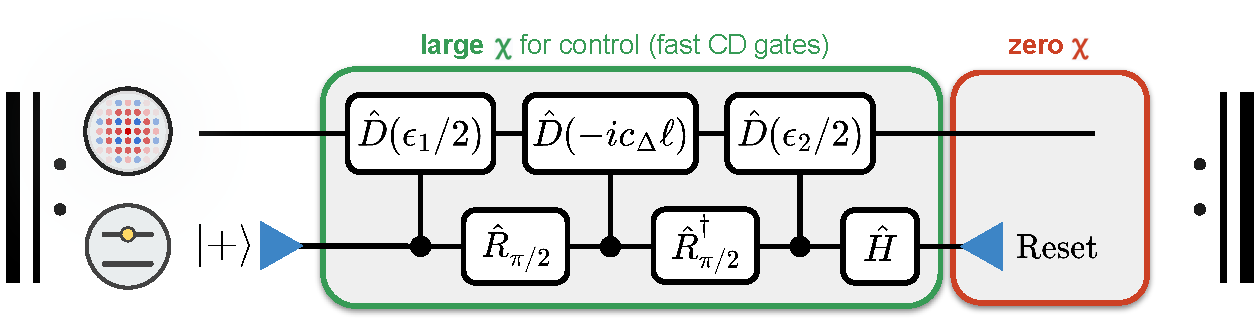
\includegraphics[width=0.85\linewidth]{Figures/4/SBS_Control_and_Reset.pdf}
    \caption[Control and reset phases of the open-loop GKP error correction.]{GKP open-loop error correction consists of two sections: control (green) and reset (red). For control, we want large $\chi$ to get fast conditional displacements. For reset, we want $\chi = 0$ to minimize backaction on the storage mode.}
    \label{fig:4_SBS_Control_and_Reset}
\end{figure}

In addition to having a large dynamic-range for the dispersive shift over some given set of external fluxes, we also wish to minimize the Kerr nonlinearities $K_g$ and $K_e$ since these terms are detrimental for bosonic QEC. Finally, we wish to be in the \textit{heavy-regime} of the fluxonium with $E_J \gg E_C$ in order to benefit from the bit-flip protection of the heavy fluxonium, which is the main reason that we are using this qubit in the first place. Simultaneously achieving all the conditions above requires us to do a multi-dimensional parameter optimization. We discovered, however, that it is possible to engineer the system to meet these requirements by carefully choosing the storage mode frequency to be \textit{between} the two sets of so-called fluxonium plasmon transitions, which are the transitions from the states $\ket{g}, \ket{e}$ to the higher excited states of the two wells, $\ket{f}$ and $\ket{h}$. At half-flux, the coupling between these plasmon states results in an avoided crossing (i.e., an energy gap), which we can use to engineer the dispersive shift $\chi(\varphi_{\rm ext})$ by placing $\omega_{gf} < \omega_s < \omega_{gh}$ and $\omega_{ef} < \omega_s < \omega_{eh}$. We refer to this condition as  \textbf{bosonic mode threading}, since the storage is 
\textit{threaded} through the gap between the two plasmon states. In our numerical simulations, we found that the bosonic mode threading condition results in $\chi(\varphi_{\rm ext})$ crossing through zero (for $E_J, E_C, E_L$ in the right range), and also minimizes the effective Kerr nonlinearity. By numerically investigating Eq. \eqref{eq:4_3DGKP_StorageQubit_H} using threading as a guideline, we ultimately settled on the parameters $\omega_s/2\pi = 8.907$ GHz, $E_J/h = 8.74$ GHz, $E_C/h = 1.69$ GHz, $E_L/h = 0.5$ GHz, and coupling strength $g/2\pi = 24$ MHz. With these parameters, we get a flux-tunable dispersive shift that can be tuned from -1 to +1 MHz in the flux range of interest, as well as reasonably low Kerr nonlinearities satisfying $K_i/\chi \lesssim 5\times 10^{-3}$ for $i \in \{g, e\}$ [cf. Fig \ref{fig:4_3D_GKP_Theory_ChiKerr}]. 

\begin{figure}[h]
    \centering
    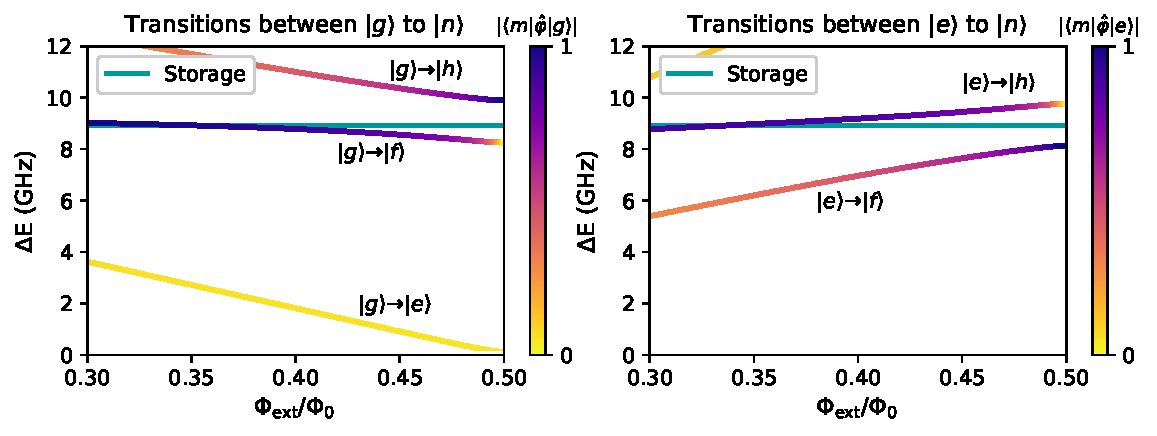
\includegraphics[width=0.93\linewidth]{Figures/4/3D_GKP_Theory_Spectrum.pdf}
    \caption[Simulated energy spectrum obtained from numerical diagonalization of the fluxonium Hamiltonian for 3D-GKP experiment.]{Energy spectrum obtained from numerical diagonalization of the fluxonium Hamiltonian with $E_J/h = 8.74$ GHz, $E_C/h = 1.69$ GHz, $E_L/h = 0.5$ GHz. The transitions $\ket{g/e}\to\ket{n}$ are colored by their phase matrix elements. We overlay the storage frequency $\omega_s/2\pi = 8.907$ GHz and see that it is \textit{threaded} between the two sets of plasmon transitions.}
    \label{fig:4_3D_GKP_Theory_Spectrum}
\end{figure}
\begin{figure}[h]
    \centering
    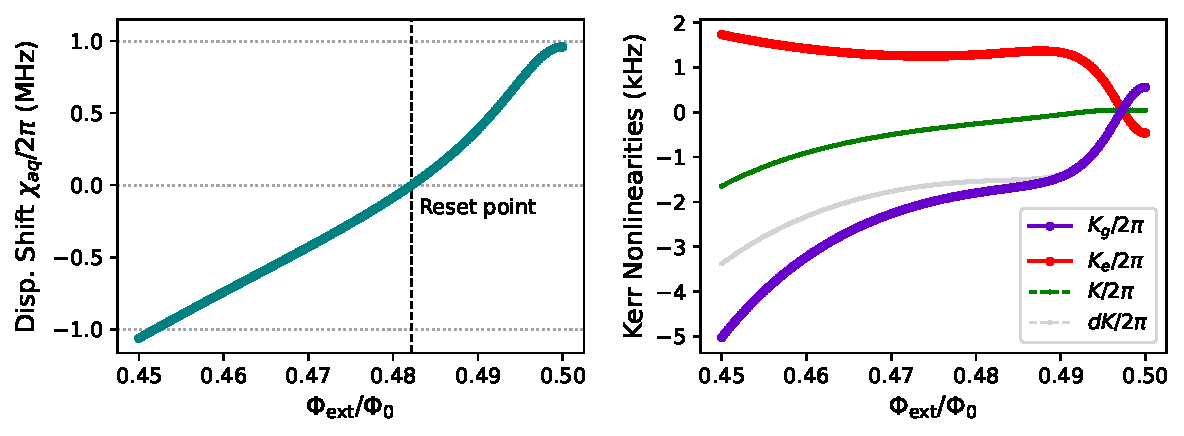
\includegraphics[width=0.93\linewidth]{Figures/4/3D_GKP_Theory_ChiKerr.pdf}
    \caption[Simulated dispersive shift and Kerr nonlinearities obtained from numerical diagonalization of the resonator-fluxonium system using the parameters of the 3D-GKP experiment.]{Left: Storage dispersive shift $\chi(\varphi_{\rm ext})$ obtained from numerical diagonalization of Eq. \eqref{eq:4_3DGKP_StorageQubit_H}. We see $\chi$ tunes with flux and crosses through zero at $\Phi_{\rm ext} \approx 0.483\Phi_0$, which is where we would perform reset. Right: Storage Kerr nonlinearities $K_g$ and $K_e$ when qubit is in $\ket{g}$/$\ket{e}$ respectively. We also plot $K = [K_g+K_e]/2$ and $dK = [K_g-K_e]/2$.}
    \label{fig:4_3D_GKP_Theory_ChiKerr}
\end{figure}

\clearpage
\section{Hardware and Setup\label{sec:4_Hardware_and_Setup}}

\subsection{3D Cavity-Fluxonium Architecture \label{sec:4_3D_Cavity_Resonators}}
To implement the proposed experiment above, we designed a package consisting of three superconducting 3D post cavities fabricated from high-purity (``5N5'') aluminium, as well as a PCB and interconnect module on which we mounted two fluxonium qubit chips. We refer to the three cavity resonators as ``A'', ``B'', and ``C'' from left to right; cavity B serves as the storage resonator, while cavities A and C serve as readout resonators for the qubits [see Fig. \ref{fig:4-3DGKP-schematic-1}(b)]. We designed the package in this way to be able to screen multiple fluxonium devices per cooldown. The chips themselves were fabricated at MIT Lincoln Laboratory out of aluminium on an 8" Si wafer, while the cavity and housing were fabricated at MIT, and then later cleaned and etched in the MIT.nano cleanroom. For additional details about the cavity fabrication, see Appendix \ref{ch:AppB}. A schematic diagram summarizing the fluxonium chip design is shown in Fig. \ref{fig:4-3DGKP-schematic-2} below.

\begin{figure}[h]
    \centering
    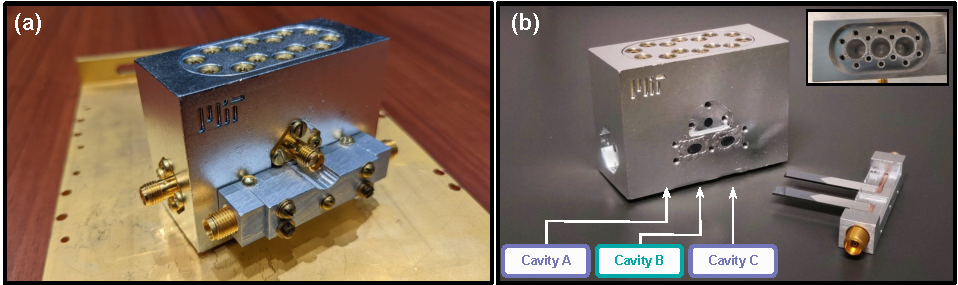
\includegraphics[width=0.95\linewidth]{Figures/4/3DGKP-Schematic-1.pdf}
    \caption[Hardware overview of 3D cavity architecture, showing both the assembled and disassembled packages.]{\textbf{(a)} Assembled 3D cavity-fluxonium package. \textbf{(b)} Disassembled view showing qubit chips glued to the interconnect module and wirebonded to a PCB for signal delivery. The chips are then inserted into the chip tunnels and screwed tight with an indium seal to assemble the package. Cavities are labelled A, B, C from left to right; cavity B serves as the storage. All three cavities are driven via SMA pins (gold); the drive port is weakly coupled for the storage resonator to minimize loss and strongly coupled for the readout resonators. Inset: inner structure of the three post cavities. Each stub forms a $\lambda/4$ resonator.}
    \label{fig:4-3DGKP-schematic-1}
\end{figure}

We will refer to the specific cavity device shown in Fig. \ref{fig:4-3DGKP-schematic-1} as the ``Mark II'' cavity. Our first attempt at fabricating a 3D cavity resonator (the ``Mark I'') had low resonator lifetimes due to an unsuccessful etch process (etching is required in order to realize high quality-factors in a 3D cavity; see App. \ref{ch:AppB}). All of the fluxonium experiments in this thesis were performed using the Mark II. Before inserting the qubit, however, we performed cryogenic measurements of the bare cavities in order to characterize their coherence. We measured the lifetime of the storage resonator to be $T_1 \approx 765$ $\mu$s, which we extracted from a fit of the resonator response to a reflection measurement using a Vector Network Analyzer (VNA). For more details about such resonator measurements, see App. \ref{ch:AppA}. Later, after optimizing our etch process, we also fabricated a ``Mark III'' cavity; while we did not use it for any of the experimental results shown in this chapter, the Mark III was helpful to have for later debugging. The bare storage lifetime in \textit{this} cavity was found to be in excess of $T_1 \approx 3$ ms. 

\begin{figure}[h]
    \centering
    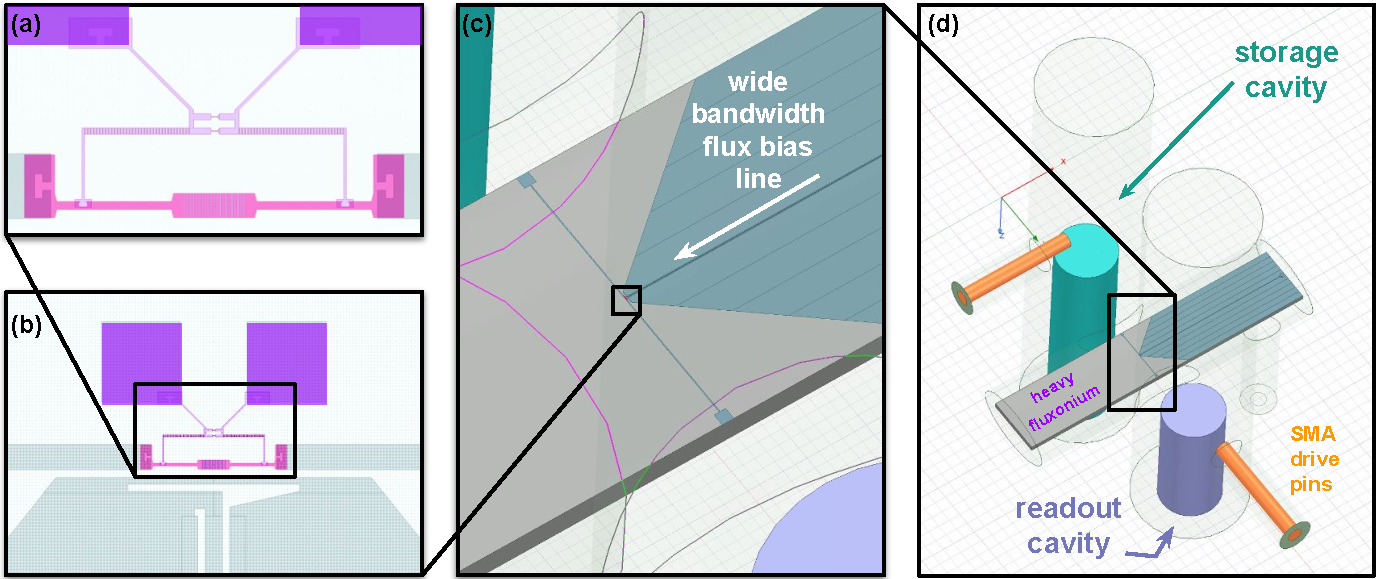
\includegraphics[width=\linewidth]{Figures/4/3DGKP-Schematic-2.pdf}
    \caption[Schematic of the fluxonium chip used in the 3D cavity architecture.]{Schematic of qubit chip in the 3D cavity architecture. \textbf{(a,b)} Fluxonium design showing capacitor pads (purple) and a shared superinductance with an auxiliary \textit{antenna} mode (pink). The antenna pads are then extended to the chip edge to implement coupling to the post cavities; the fluxonium-resonator couplings are thus mediated via the antenna. \textbf{(c)} The fluxonium is flux biased using an on-chip wideband flux line capable of delivering both radio-frequency (RF) and DC signals; the flux line terminates in a loop (cf. panel b) and the current returns via the ground plane (teal blue in panel c, representing aluminium metallization on the chip). \textbf{(d)} Chip integrated in 3D cavity showing the chip edge partially extending into both the storage and readout cavities (teal and lilac posts, respectively) to implement couplings. The schematic in panel d focuses on a single storage-qubit-readout subsystem of the package; the full system includes another qubit and readout (cf. Fig \ref{fig:4-3DGKP-schematic-1})}
    \label{fig:4-3DGKP-schematic-2}
\end{figure}

%\todo{Fitting to get pin lengths.}


\subsection{Cryogenic Setup}

The experiments were performed using a Leiden CF-CS81 dilution refrigerator operated at base temperatures of 8-10 mK. The fridge consists of five temperature stages\footnote{The fridge temperature is primarily tracked using three 1 k$\Omega$ platinum (PT-1000) thermometers at the 50K, 3K, and MXC plates. The 3K plate also has a 10 k$\Omega$ RuO$_2$ sensor, while the MXC has additional resistive and CMN magnetic susceptibility thermometers. We note that the fridge has high-power heaters at the 50K and 3K stages for fast warm-ups, and also features a liquid nitrogen pre-cooling circuit for fast cooldowns.} as shown in Fig. \ref{fig:4-fridge-wiring}, as well as seven shielding cans that each thermalize to a different temperature stage (not pictured). Specifically, we have two vacuum cans thermalized to room temperature and 1K respectively, and three other cans for additional electromagnetic shielding. We mount devices on a ``cold finger'' that is thermalized to the mixing chamber (MXC) and encapsulated in a mu-metal shield to protect against infrared radiation and stray magnetic fields. A timelapse video of the process to install these various shields can be found \href{https://youtu.be/KkvUc9Aw77s?t=829}{\textbf{here}}. 

\begin{figure}[h]
    \centering
    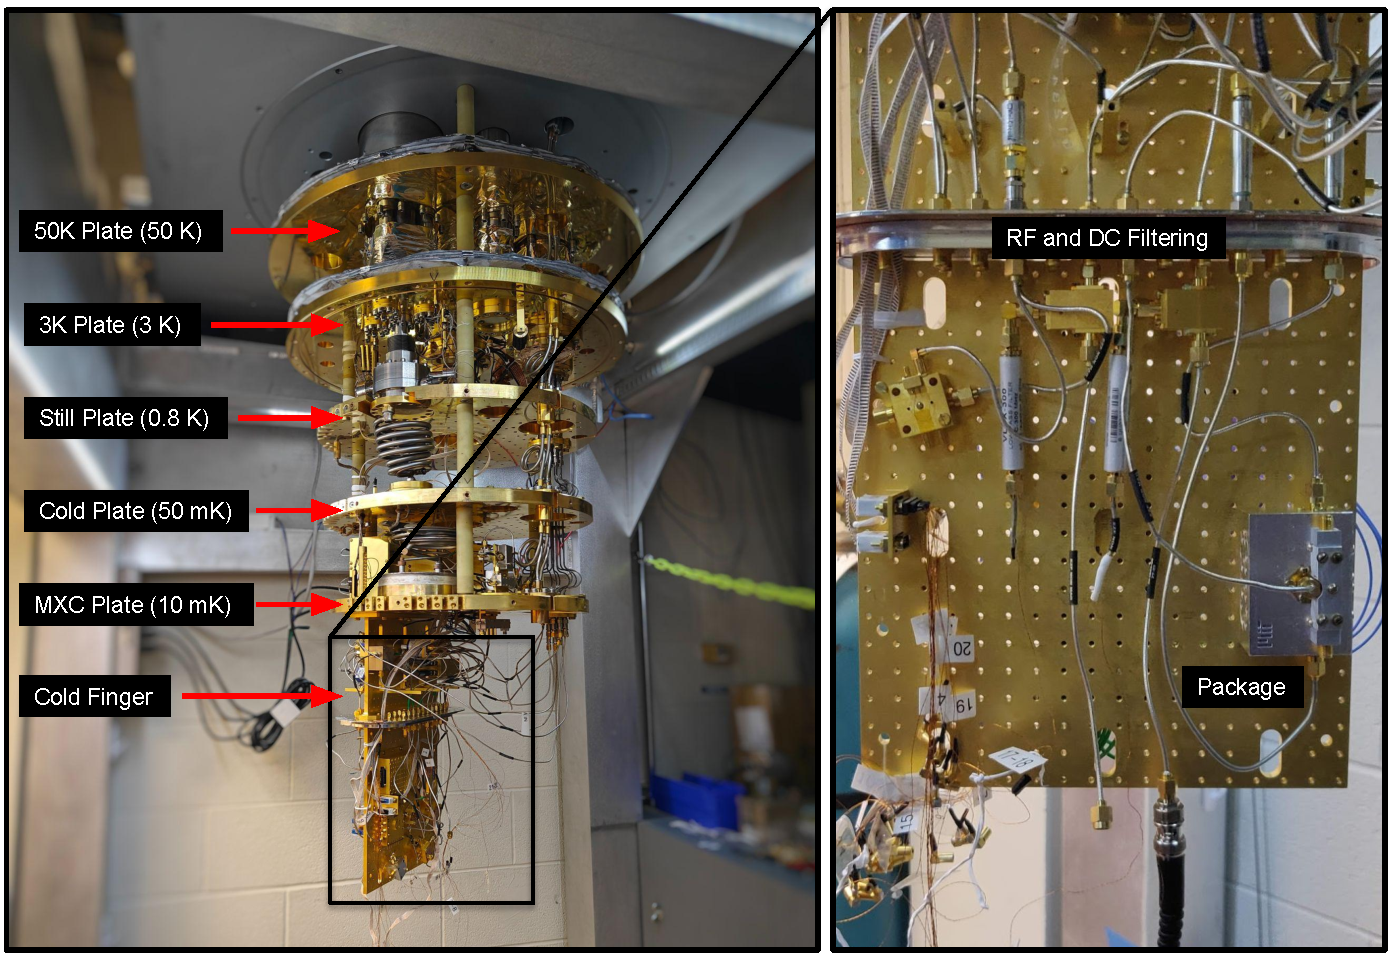
\includegraphics[width=0.9\linewidth]{Figures/4/Fridge-Wiring.pdf}
    \caption[Internal structure of the Leiden CF-450 dilution refrigerator used for the experiments in this thesis.]{Left: Internal structure of the Leiden CF-450 dilution refrigerator used for the experiments in this thesis. The fridge consists of several plates/stages each thermalized to successively colder temperatures. Right: Devices are mounted onto a ``cold finger'' that is thermalized to the mixing chamber (MXC) plate at 10 mK.}
    \label{fig:4-fridge-wiring}
\end{figure}
\clearpage

The specific experiments presented in this thesis used both DC and radio-frequency (RF) microwave lines to deliver signals to the 3D cavity and fluxonium package. We used three microwave ``drive'' lines for the two fluxonium qubits and the storage resonator, as well as two DC twisted pair connections to provide static flux biasing for the two qubits. The qubit RF and DC signals were first individually filtered and then combined at the mixing chamber through an RF choke. We filtered the DC component using a Mini-Circuits VLFX-300+ low-pass filter, while the RF component was filtered via a K\&L Microwave 12 GHz low-pass filter. This configuration allowed us to probe the higher level transitions of the fluxonium via two-tone spectroscopy through the qubit drive line. 

To attenuate thermal noise coming from the room temperature setup, several attenuators were placed along each of the input microwave lines: a total of 50 dB for the ``drive'' lines and 70 dB for the ``readout'' line. The readout setup had several salient features worth noting: firstly, we used just a single microwave line connected to the two readout cavities via microwave switch; by setting the switch configuration, we selected which of the cavities to measure. Secondly, we used circulators to measure the cavity resonances in reflection. Finally, the reflected output readout signal was pre-amplified using a Josephson travelling wave parametric amplifier (TWPA) at the MXC stage, before being further amplified by a low-noise high-electron-mobility transistor (HEMT) amplifier at 3K, and then a room temperature MITEQ amplifier. The full wiring schematic for this setup is shown below in Fig. \ref{fig:4-microwave-wiring-diagram}. 

At room temperature, pulse waveforms for the various elements were generated using an OPX+ controller from Quantum Machines. For the storage drive, we used an Agilent PSG Signal Generator (E8267D) from Keysight to supply an RF signal which was then combined with the intermediate-frequency (IF) signal from the OPX using the PSG's internal wide-bandwidth IQ mixer. The qubit drive was produced similarly, using a separate Agilent PSG Signal Generator. When performing low-frequency two-tone spectroscopy of the fluxonium $g$--$e$ transition, however, we bypassed the Agilent and instead used baseband signals in the 0-350 MHz range directly from the OPX. Finally, the readout resonator IF signals were generated via the OPX and then passed into a Rohde and Schwarz SGS100A SGMA RF source for upconversion using an internal IQ mixer. The local oscillator (LO) reference signal used for IQ modulation was also passed on to a separate external IQ mixer to demodulate the readout RF output signal coming out of the fridge. The demodulated intermediate-frequency I and Q components were then digitized and processed using the FPGA within the OPX. All microwave signal generators were frequency-locked via a common 10 MHz rubidium clock. 

The DC signals used for static flux biasing were generated via a Yokogawa GS200 Voltage/Current source operated in ``Voltage'' mode; this was then sent into the Qdevil breakout board and then into the fridge via a Fisher cable. Once in the fridge, the signal lines were passed through a resistive DC low-pass filter before terminating in a twisted pair connection. When operating a Yokogawa (or ``Yoko'') in Voltage mode, the DC signal is typically routed through a 1-10 k$\Omega$ resistor to produce an associated current; anecdotally around our lab, this has also been reported to help reduce flux noise from DC lines. However, in the experiments reported below, we mostly chose not to do this and instead used only the bare resistance of the DC line when connected to the fluxonium device, which we measured to be 152.5 $\Omega$ using a multimeter when the fridge was cold. This allowed us to generate a larger current for a given voltage. As we discuss in Sec. \ref{sec:4_Time_Domain}, we later also measured the flux noise amplitude of the qubit when using the ``Current'' mode of the Yoko and found negligible differences in the results. % \todo: check DC low-pass filter

\begin{figure}[ht]
    \centering
    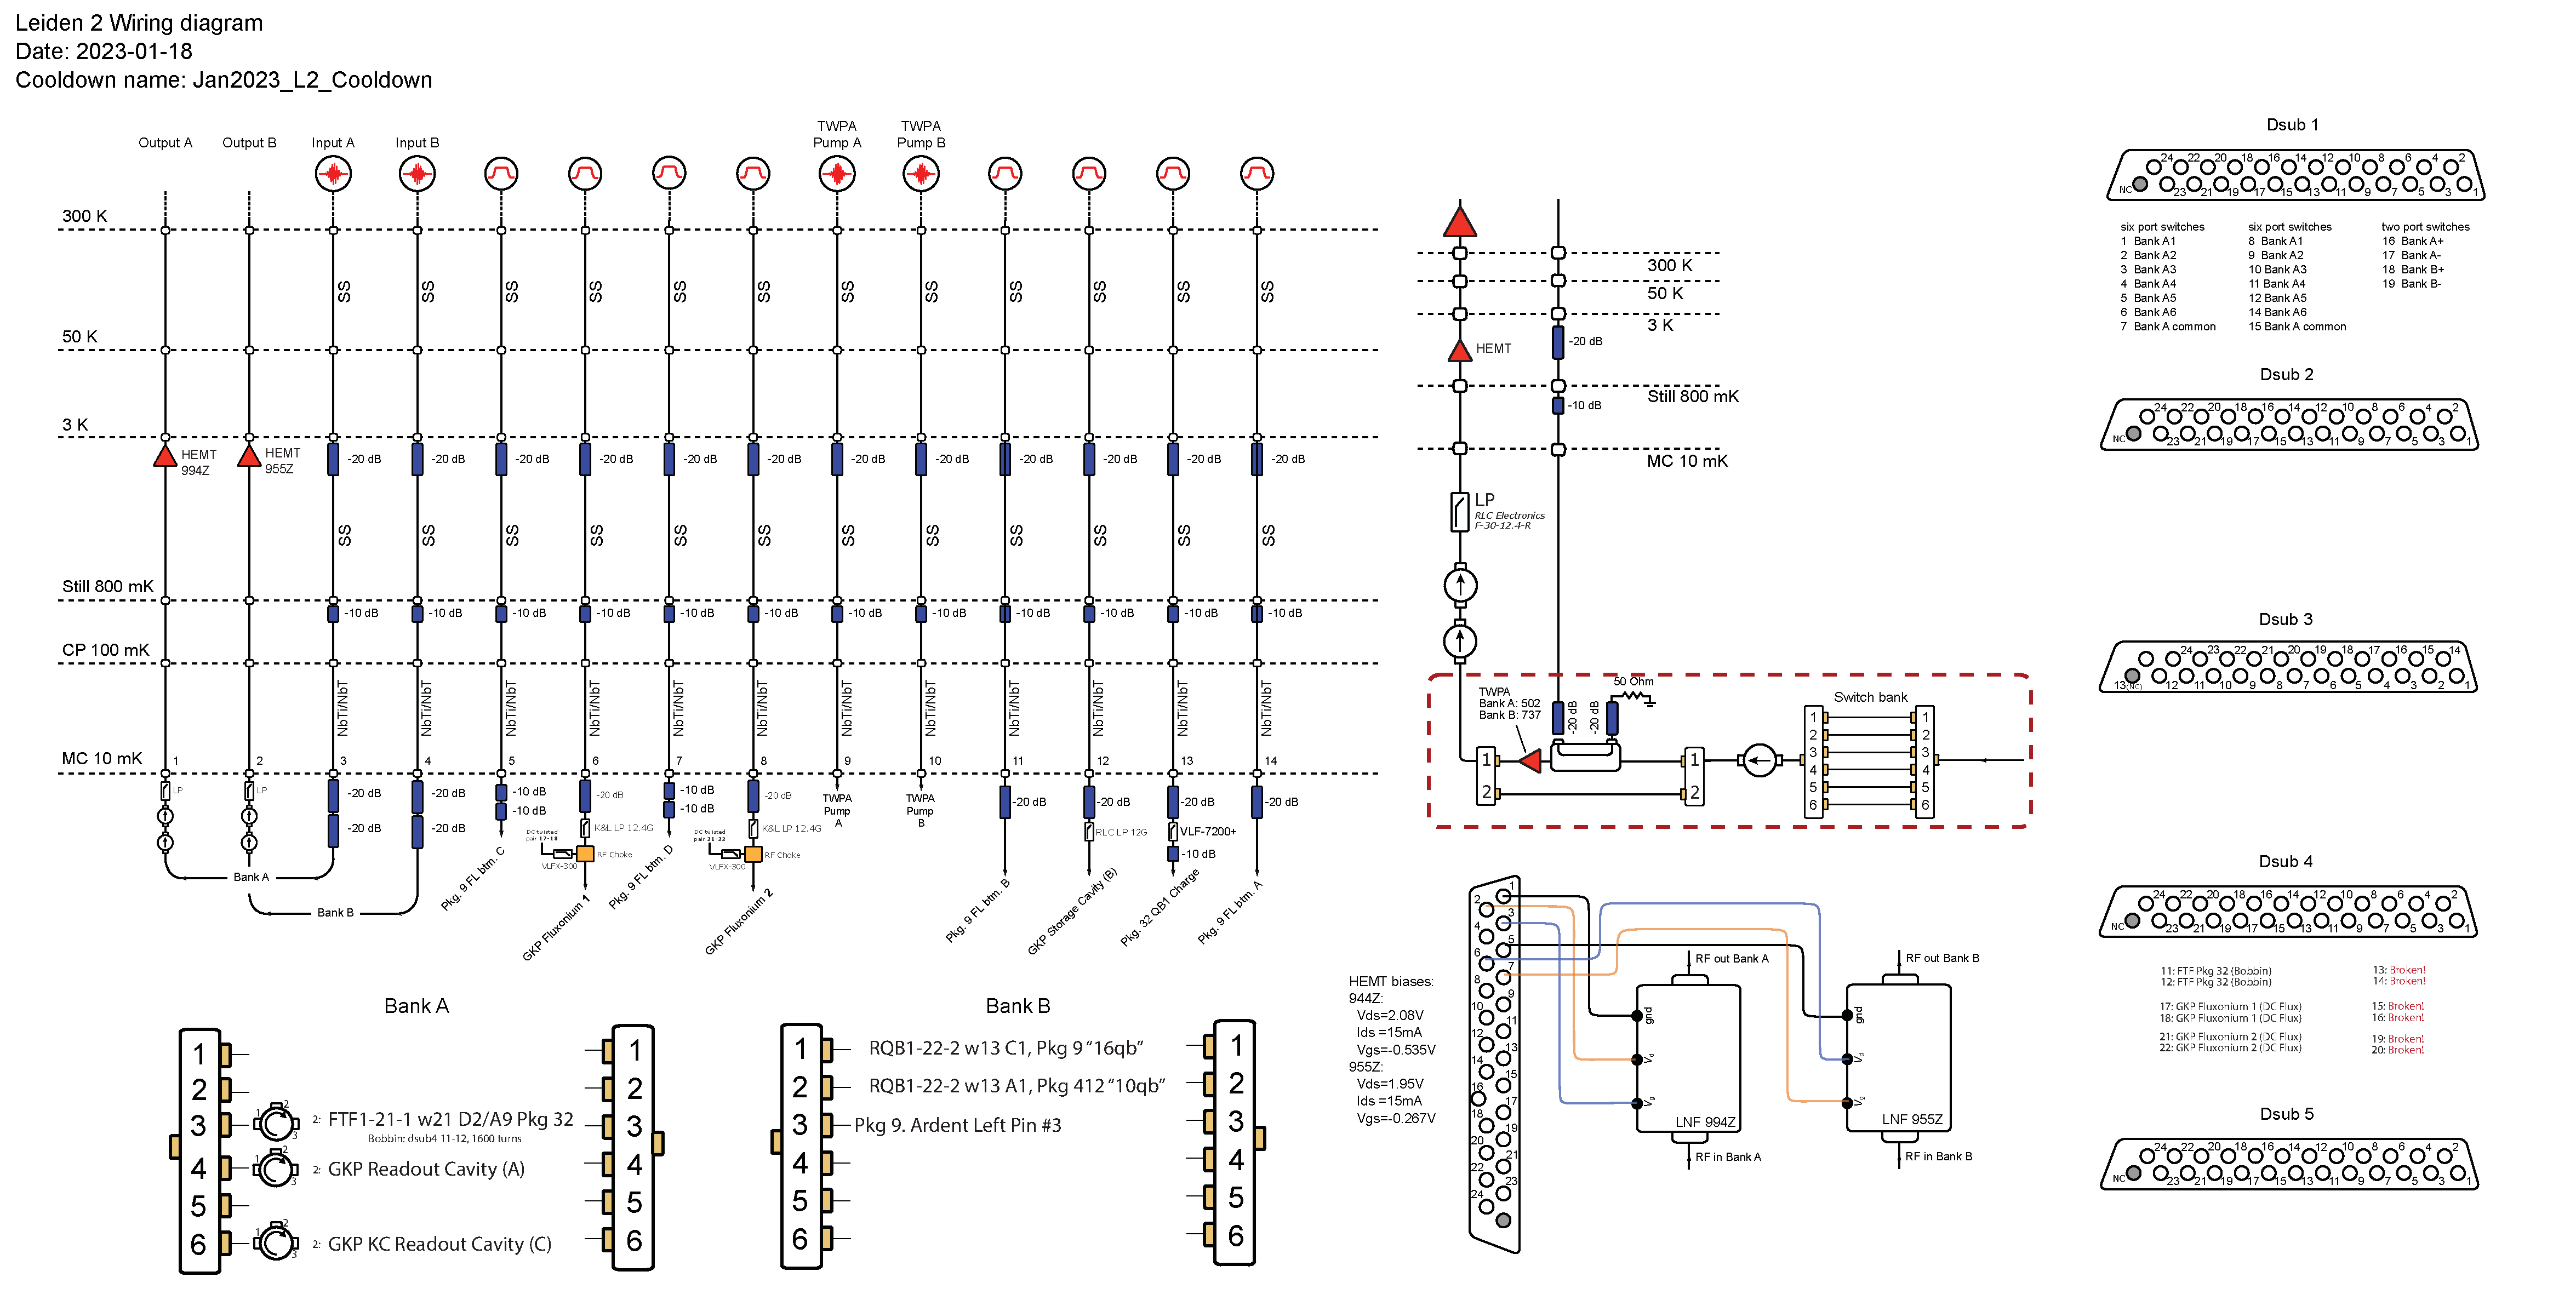
\includegraphics[width=\linewidth]{Figures/4/Microwave-Wiring-Diagram.pdf}
    \caption[Microwave wiring diagram for the experiment.]{Wiring diagram for the experiment consisting of a readout chain set up in a reflection configuration and RF drives for the fluxonium qubit and storage resonator. We combine the qubit RF signal with a DC bias at the mixing chamber using an RF choke.}
    \label{fig:4-microwave-wiring-diagram}
\end{figure}


\clearpage
\section{Resonator and Two-Tone Spectroscopy\label{sec:4_Resonator_and_Two_Tone}}

In this section, we will present experimental results from our first 3D cavity-fluxonium device with a GKP1 fluxonium chip in our Mark II cavity. We begin with a spectroscopic characterization of the readout resonator and qubit here, followed by time-domain measurements of the qubit in Sec. \ref{sec:4_Time_Domain}, and finally discuss storage resonator measurements in Secs. \ref{sec:4_StorageChi} and \ref{sec:4_StorageCoherenceProblems}. Unless stated otherwise, all data in the upcoming sections was taken using readout cavity A and its associated fluxonium chip. We therefore restrict our focus to the subsystem of the Mark II cavity-fluxonium package comprised of cavity A (readout resonator), fluxonium A (qubit), and cavity B (storage resonator).

\subsection{Resonator Spectroscopy}
In most circuit QED experiments, the readout resonator forms a crucial gateway through an experimenter probes the system of interest. To this end, the first measurement step we took after cooling down our device was to locate the readout resonator via spectroscopy. As discussed in Sec. \ref{sec:4_3D_Cavity_Resonators}, the readout pin length was chosen here to be overcoupled, with a target coupling rate of $\kappa_c/2\pi \approx 10$ MHz. We were thus able to locate the cavity resonance fairly easily using the VNA and later via pulsed resonator spectroscopy on the OPX with a 10 $\mu$s pulse [see Fig. \ref{fig:4_resonator_spectroscopy}(a)].
\begin{figure}[h]
    \centering
    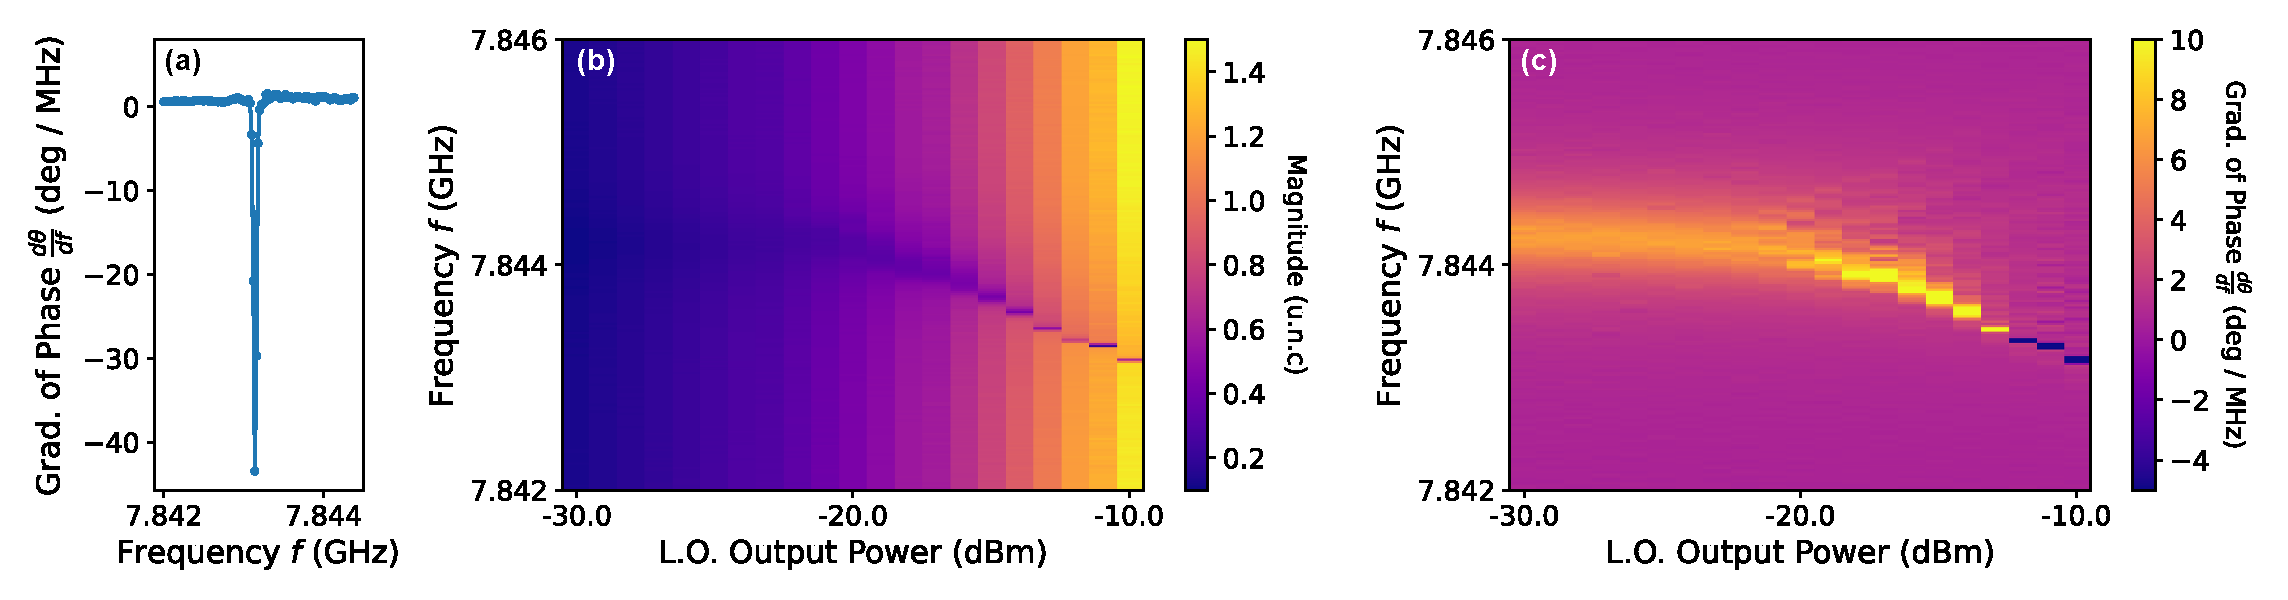
\includegraphics[width=\linewidth]{Figures/4/resonator_spectroscopy.pdf}
    \caption[Resonator spectroscopy experiments showing a single resonator spectrum and a sweep vs. drive power.]{\textbf{(a)} Readout cavity resonance measured using a time-domain resonator spectroscopy sequence. We plot the gradient of the phase $\theta$ of the reflected signal. \textbf{(b,c)} Sweep of resonator spectroscopy vs. drive power; here we plot both the magnitude and phase.}
    \label{fig:4_resonator_spectroscopy}
\end{figure}

We next repeated pulsed resonator spectroscopy as a function of the input power of the resonator tone to realize a so-called ``punchout'' measurement [Fig. \ref{fig:4_resonator_spectroscopy}(b-c)]. In the data, we observe the resonator ``punching'' out, i.e., its frequency shifting downwards towards its bare value as we increase the drive power as it decouples from the nonlinear degrees of freedom in the system (e.g., the qubit or antenna mode here). Punchout is typically used as a way to check whether a qubit is present, since the nonlinearity of the qubit directly results in a nonlinear response in the resonator. For a practical explanation of this, I refer interested readers to Ref. \cite{naghiloo2019introduction} which also gives a step-by-step experimentalist's introduction to qubit measurements in circuit QED. 

Due to its coupling to the fluxonium qubit, we also expect the resonator to inherit some flux dependence in addition to nonlinearity. Therefore, after verifying that the resonator frequency changes with power, we next performed resonator spectroscopy vs. the applied external flux bias on the qubit [see Fig. \ref{fig:4_resonator_spectroscopy_vs_flux}]. We set the bias using the room temperature Yokogawa source to set voltage (which induced a current through the DC line, and in turn generated an applied flux through the fluxonium loop). After setting each bias voltage, we waited for 0.1s for the flux to settle and then performed resonator spectroscopy.  

\begin{figure}[h]
    \centering
    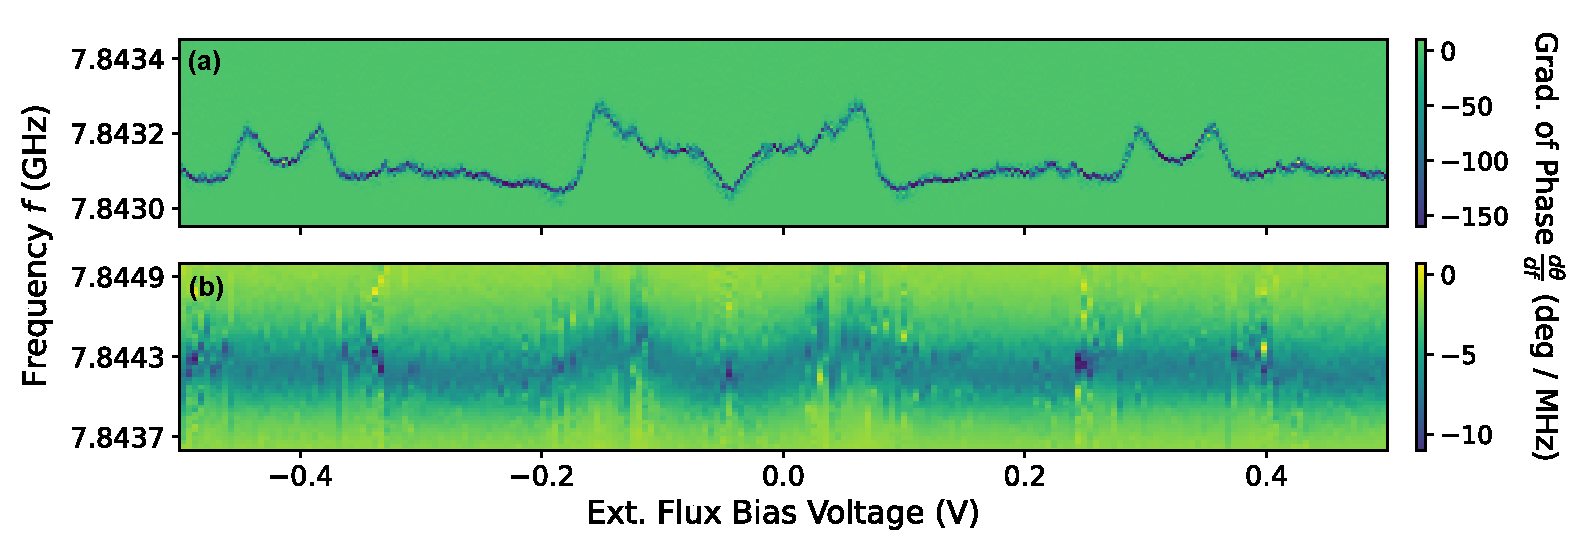
\includegraphics[width=\linewidth]{Figures/4/resonator_spectroscopy_vs_flux.pdf}
    \caption[Resonator spectroscopy vs. external applied flux on the fluxonium qubit.]{Resonator spectroscopy vs. external bias voltage on the qubit. The top panel shows high-power data with an LO output power [cf. Fig. \ref{fig:4_resonator_spectroscopy}] of -10 dBm, while bottom panel shows lower-power data taken at -30 dBm. We see the resonator spectrum is indeed periodic with the bias voltage.}
\label{fig:4_resonator_spectroscopy_vs_flux}
\end{figure}

We see that the the resonator frequency indeed varies periodically with the bias voltage. From the periodicity of the spectrum, we found (and later corroborated via qubit two-tone spectroscopy measurements) that a flux quantum in this device corresponds to 4.872 mA, realized in this configuration via a voltage of about 0.743 V applied over the line resistance of 152.5 $\Omega$. The resonator spectrum is expected to be symmetric about both zero external flux ($\Phi_{\rm ext} = 0$) and ``half-flux'' ($\Phi_{\rm ext} = \Phi_0/2$), and we can observe two symmetry points above --- one at $V_b \approx -0.045$ V, and other at both $V_b \approx 0.326$ V and $V_b \approx -0.414$ V. From the averaged data in Fig. \ref{fig:4_resonator_spectroscopy_vs_flux} alone, it is rather difficult to identify which of these symmetry points corresponds to ``half-flux''. However, we can make this identification by instead working with single-shot data, i.e., not directly averaging across shots on the OPX during readout. At $\Phi_{\rm ext} = 0$, the fluxonium has a single ground state $\ket{g}$ that the qubit relaxes to in thermal equilibrium. Thus the dispersive readout will result in a \textit{single} ``I-Q blob'' in the demodulated signal. However, at $\Phi_{\rm ext} = \Phi_0/2$, both the ground and excited states will be thermally occupied in equilibrium due to the low-frequency nature of the qubit \cite{manenti2023quantum}, and thus we expect to see two ``blobs'' in the I-Q plane corresponding to the qubit initial state being in either $\ket{g}$ or $\ket{e}$. When we set the Yoko voltage to $V_b = -0.04465$ V, the single-shot data [cf. Fig \ref{fig:4_single_shots}] reveals two IQ ``blobs'' in the histogram, confirming that this bias point is, in fact, the half-flux sweet spot. (By association, the other symmetry points correspond to \textit{integer} flux quanta). Using this calibration of the flux axis, we can map between the bias voltage and the applied external flux $\Phi_{\rm ext}$ in all subsequent measurements. 

\begin{figure}[h]
    \centering
    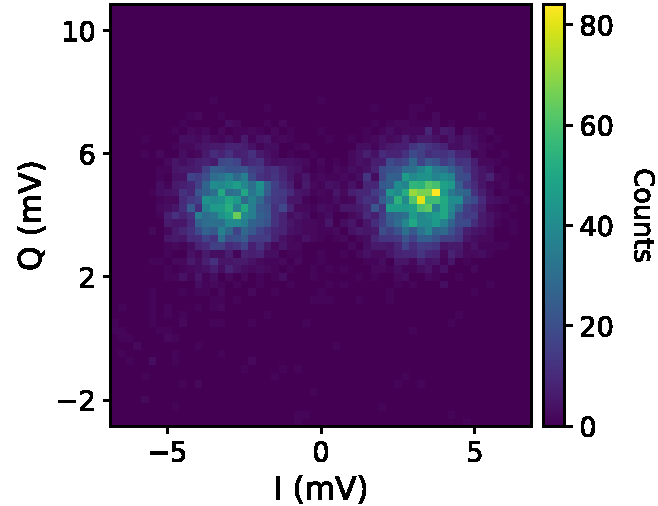
\includegraphics[width=0.51\linewidth]{Figures/4/single_shots.pdf}
    \caption[Readout I-Q histogram showing two characteristic readout ``blobs'' when the fluxonium is parked at half-flux.]{Histogram of 10,000 digitized single-shot readout measurements, plotted in the I-Q plane. The two ``blobs'' correspond to the two qubit states $\ket{g}$ and $\ket{e}$ that will both be populated in equilibrium when the fluxonium is parked near the half-flux sweet spot.}
\label{fig:4_single_shots}
\end{figure}


\newpage
\subsection{Two-Tone Spectroscopy}
After characterizing the resonator, our next step was \textit{two-tone spectroscopy} (also called qubit spectroscopy). Here, the two ``tones'' in question are (i) a qubit drive tone to probe transitions of the fluxonium, followed by (ii) a resonant readout tone. Practically, we can understand a two-tone spectroscopy experiment as follows by considering the dispersive Hamiltonian \cite{zhu2013cQEDfluxonium}:
\begin{equation}
    \hat{H} = \sum_k \tilde{\omega}_k \op{k}{k} + \bigg(\omega_r^0 + \sum_k \chi_k \op{k}{k}\bigg) \hat{a}^\dagger\hat{a}
\end{equation}
We have Lamb-shifted qubit energies $\tilde{\omega}_k$ and eigenstates $\ket{k}$, as well as a resonator whose effective frequency $\tilde{\omega}_r$ (term in parentheses) depends on the qubit state. For the sake of illustration, let's briefly work near zero flux so that only the ground state $\ket{g}$ is initially populated in thermal equilibrium. The basic idea of the experiment is to play a weak continuous spectroscopy (or ``\textit{saturation}'') tone on the qubit. As we sweep the frequency, we will eventually come into resonance with a qubit transition, e.g., $\tilde{\omega}_{gl} = \tilde{\omega}_{l} - \tilde{\omega}_{g}$ between $\ket{g}$ and some other state $\ket{l}$. When this happens, the resonant tone has the effect of driving Rabi oscillations between the states $\ket{g} \leftrightarrow \ket{l}$; furthermore, over many multiples of the coherence time, the qubit state will also change due to decoherence processes (i.e., $T_1$ relaxation and heating, as well as dephasing). The qubit will thus be left in a non-equilibrium steady state $\hat{\rho}$ with occupation probabilities $p_k$. Due to the dispersive interaction, this mixed state in turns leads to an average resonator frequency
\begin{equation}
    \ev{\tilde{\omega}_r}_{\rm final} = \omega_r^0 + \Tr\bigg(\hat{\rho} \sum_k \chi_k \op{k}{k}\bigg) = \omega_r^0 + \sum_k p_k \chi_k
\end{equation}
that is different from the initial one: $\ev{\tilde{\omega}_r}_{\rm init} = \omega_r^0 + \chi_g$. Using a resonator measurement, we can then detect this change in the resonance frequency (e.g., by measuring the change in signal phase when ``reading out'' at a fixed frequency $\ev{\tilde{\omega}_r}_{\rm init}$), and so map out the qubit transitions. If we now do this as a function of flux, the initial qubit state may also need to be described by a mixed state, e.g. a thermal mixture of $\ket{g}$ and $\ket{e}$ near half-flux; nevertheless, as long as the initial and final mixed states lead to different average resonator frequencies, we will be able to identify that a transition has occurred. 

In experiment, we performed wideband two-tone spectroscopy to map out the higher energy transitions of the fluxonium versus external flux. The full spectrum is shown below in Fig. \ref{fig:4_two_tone_vs_flux_full}; we already see a rich set of features in the data. The qubit transitions have a clear dependence on flux, and are notably symmetric about the two sweet spots at $\Phi_{\rm ext} = 0$ and $\Phi_{\rm ext} = \Phi_0/2$. In panel (b), we overlay a theoretical prediction obtained from numerical diagonalization of the fluxonium Hamiltonian with free parameters $E_C$, $E_J$, and $E_L$. We extract
\begin{equation}
    E_C/h \approx 1.678 \,\, \text{GHz}, \quad  E_J/h \approx 8.987 \,\, \text{GHz}, \quad  E_L/h \approx 0.342 \,\, \text{GHz} 
    \label{eq:4_qubit_parameters_fit}
\end{equation}
as the qubit parameters for this device by fitting to the data. This is within the range that we designed for, and results in a qubit frequency of approximately 94.1 MHz at half-flux. 

At this resolution, there are also certain features that appear to be constant with flux. We can identify these as the various linear modes in the system, e.g. the storage resonator at 8.86 GHz, and the two on-chip antenna modes at 8.60 GHz and 8.46 GHz. Since each of these modes has a dispersive shift to the readout resonator (also shown), we are able to see them in this two-tone measurement just as we do the other qubit transitions\footnote{We can also see some other faint qubit-like transitions near half-flux. We'll comment on these later, as they are actually quite interesting: it turns out that they are two-photon ``parasitic'' qubit-resonator transitions.}. Note that each of these linear modes (including the readout) has \textit{some} flux dispersion if we zoom in close enough. This is important for readout calibration, as typically the readout frequency must be calibrated at each new flux operating point. In the data shown here, we did not do this, and instead used a constant frequency tone at 7.8442 GHz, which was approximately resonant across the entire flux range (cf. low-power data in Fig. \ref{fig:4_resonator_spectroscopy_vs_flux}). While this worked reasonably well, we nonetheless see variations in the readout contrast that could be improved by first redoing resonator spectroscopy at each flux point prior to two-tone, or by creating a lookup table ahead of time. 

From the spectrum, we also clearly see that the storage resonator frequency indeed lies in between the two sets of fluxonium plasmon transitions. This is precisely the condition we wanted to engineer in our system: as a reminder, we refer to it at bosonic mode threading. We highlight the threading condition in a zoomed-in scan below [cf. Fig. \ref{fig:4_two_tone_vs_flux_zoom}]. 

\begin{figure}[t]
    \centering
    \includegraphics[width=0.88\linewidth]{Figures/4/two_tone_vs_flux_full.pdf}
    \caption[Wideband two-tone spectroscopy showing the landscape of transitions in our 3D-cavity package.]{\textbf{(a)} Wideband two-tone spectroscopy showing the landscape of transitions in our 3D-cavity package. \textbf{(b)} Overlaid fitted theoretical predictions based on numerical diagonalization of the fluxonium Hamiltonian with free parameters $E_C$, $E_J$, $E_L$. We plot simulated qubit transitions $\ket{g/e}\to\ket{n}$ in purple/red respectively, as well as approximate frequencies of the various linear modes in the system such as the storage, readout, and antennas (shown as straight lines here). Note, due to unwanted crosstalk, we were able to measure antenna C via readout cavity A. Finally, we also highlight two-photon transitions as thin dashed lines. We will comment on these in more detail in the main text.}
\label{fig:4_two_tone_vs_flux_full}
\end{figure}
\clearpage
\begin{figure}[hp]
    \centering
    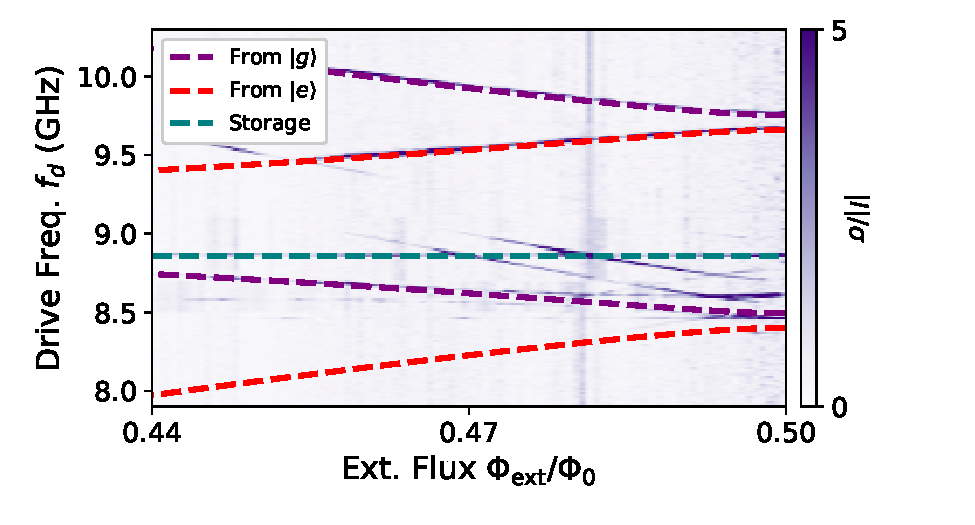
\includegraphics[width=0.73\linewidth]{Figures/4/two_tone_vs_flux_zoom.pdf}
    \caption[Zoomed-in two-tone spectroscopy showing bosonic mode threading of the storage resonator frequency between the fluxonium plasmon transitions.]{Zoomed-in two-tone spectroscopy showing bosonic mode threading, with the storage resonator frequency in between the two sets of fluxonium plasmon transitions. Dashed lines from $\ket{g}$ and from $\ket{e}$ show theoretical predictions from numerical diagonalization as before. The storage flux dispersion cannot seen at this resolution.}
\label{fig:4_two_tone_vs_flux_zoom}
\end{figure}

Our next experimental step was low-frequency qubit spectroscopy near half-flux using a direct baseband drive to map out the qubit  $\ket{g}\to\ket{e}$ transition: we show the data below in Fig. \ref{fig:4_qubit_spectroscopy}. Unlike prior measurements, here we used a dual readout post-selection scheme \cite{ding2023FTF} to improve contrast and assign an occupation probability to the qubit. This was crucial to obtain our results, and we will discuss it further in the upcoming section.

\begin{figure}[h]
    \centering
    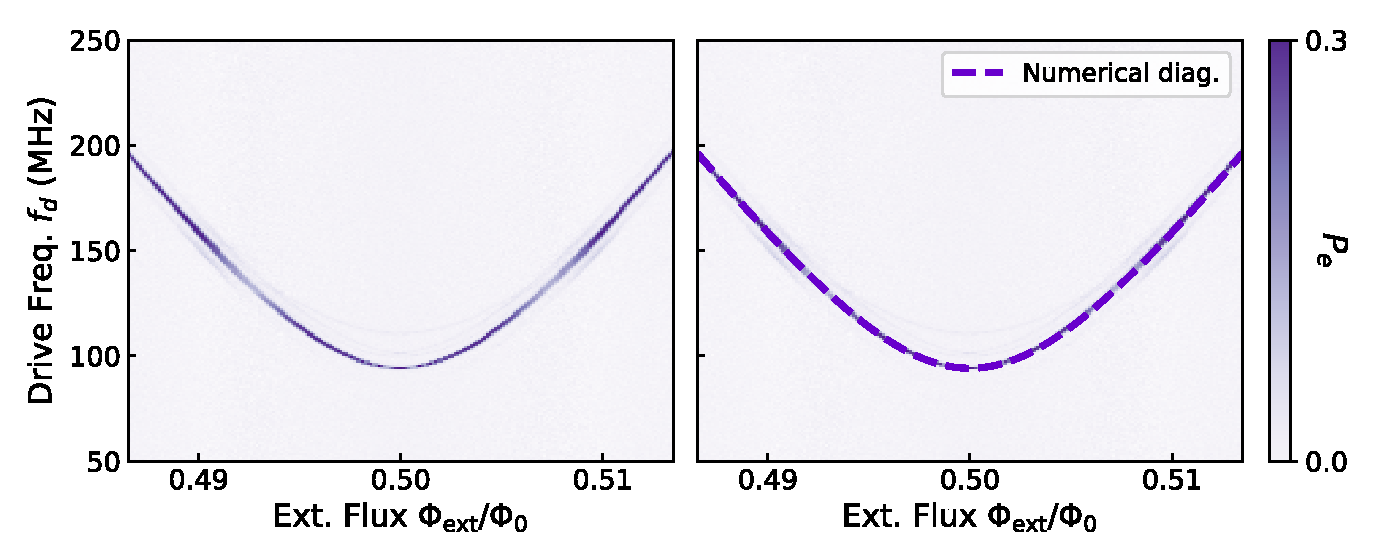
\includegraphics[width=0.88\linewidth]{Figures/4/qubit_spectroscopy.pdf}
    \caption[Baseband two-tone spectroscopy showing the fluxonium qubit $\ket{g}\to\ket{e}$ transition.]{Post-selected baseband two-tone spectroscopy showing the fluxonium $\ket{g}\to\ket{e}$ transition with and without the theoretical fit from numerical diagonalization using the same parameters as before [Eq. \eqref{eq:4_qubit_parameters_fit}]. At half-flux, the qubit frequency is 94.1 MHz.}
\label{fig:4_qubit_spectroscopy}
\end{figure}

\section{Time-Domain Measurements of the Qubit \label{sec:4_Time_Domain}}

\subsection{Post-Selection via Single-Shot Readout}

Near half-flux, the energy of the fluxonium qubit transition $\h\omega_q$ can be much smaller than the ambient temperature $k_BT$ of a typical dilution refrigerator. As a result, the fluxonium in equilibrium will be in a thermal mixture of $\ket{g}$ and $\ket{e}$; we saw this in Fig. \ref{fig:4_single_shots} already. For our specific qubit with frequency $f_q = 94.1$ MHz and assuming an effective temperature of $T = 40$ mK, the excited state population is given by a Boltzman distribution: $p_e = 1 / (e^{+\h\omega_q/k_B T} + 1) \approx 47\%$. For the higher-level (i.e., wideband) two-tone spectroscopy above, this initial thermal distribution was not a problem --- on the contrary, starting from a mixed state is even beneficial, allowing us to see transitions out of both $\ket{g}$ and $\ket{e}$. However, for baseband qubit spectroscopy probing the $\ket{g}\leftrightarrow\ket{e}$ transition, and critically also for time-domain experiments, this ceases to be true. For these measurements, we instead want to be able to discriminate between the two states. In our experiments, the approach we chose to do this was single-shot readout and post-selection. We specifically followed the dual readout scheme discussed in Refs. \cite{ding2023FTF, ding2023thesis} (cf. Fig. \ref{fig:4_postselection} below)\footnote{At this point, I'd also sincerely like to thank Leon Ding for his early guidance with fluxonium experiments!}. Here, the first readout pulse initializes the fluxonium state to either $\ket{g}$ or $\ket{e}$ via projective measurement. We then start the rest of the experimental sequence (e.g., qubit pulses, delays, storage pulses) from a known initial state, and finally conclude with a second readout pulse to record the qubit state. All the time-domain measurements that follow used this post-selected sequence. 

\begin{figure}[h]
    \centering
    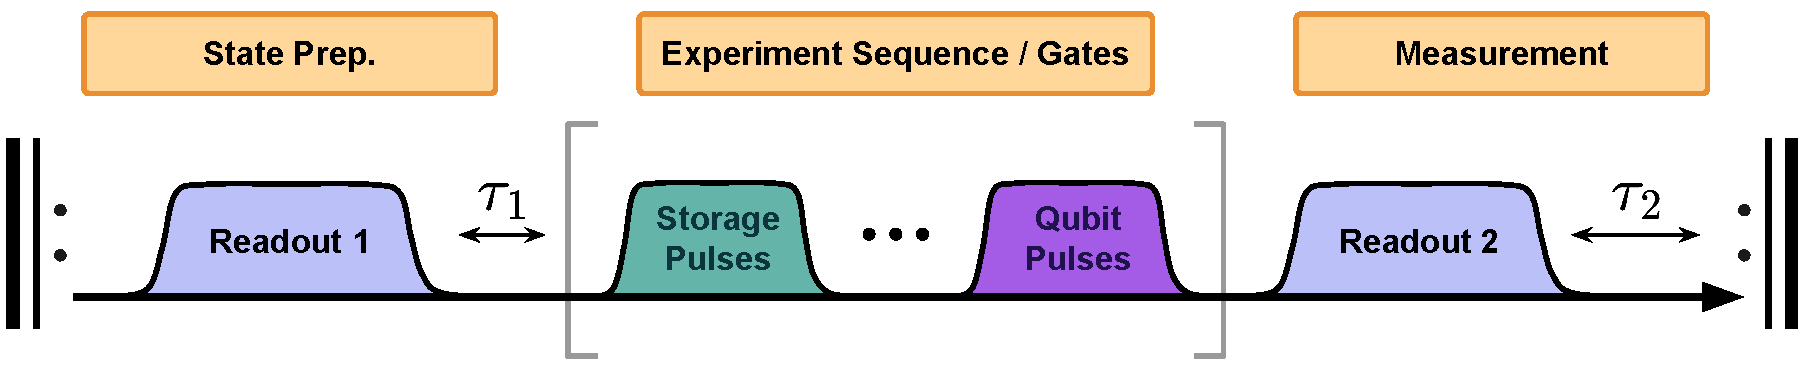
\includegraphics[width=0.9\linewidth]{Figures/4/postselection.pdf}
    \caption[Dual-readout post-selection sequence used for time-domain experiments in this thesis.]{Dual readout post-selection. Here, the first readout prepares the qubit in $\ket{g}$ or $\ket{e}$ and the second readout records the final qubit state after performing the experiment sequence. We introduce a short ring-down time $\tau_1$ to allow readout photons to decay after the first readout, and a longer delay $\tau_2$ to let the qubit relax to equilibrium between shots.}
    \label{fig:4_postselection}
\end{figure}

\subsection{Rabi Oscillations and Pi Pulse Calibration}

After having identified the qubit frequency in two-tone spectroscopy, we next turned to time-domain experiments involving coherent manipulation of the qubit state. The first of these was, of course, to demonstrate Rabi oscillations between the $\ket{g}$ and $\ket{e}$ states using a resonant drive. In heavy fluxonium, the $T_1$ protection that arises due to the small charge matrix element also has the effect of making it generically more difficult to drive the associated transitions. As a result, several previous experiments with fluxonium or other low-frequency flux qubits have had to use either non-adiabatic Landau-Zener flux control \cite{oliver2005mach, campbell2020universal, zhang2021universal}, or virtual (Raman) transitions mediated by a higher energy state \cite{earnest2018realization}. Thankfully, we were able to use more conventional microwave-based control via a resonant drive, since our device was not quite so heavy. 

In Fig. \ref{fig:4_rabi}, we show a typical power Rabi measurement, taken with the qubit parked at half-flux. For this data, we specifically used a fixed length ($\tau = 200$ ns) Gaussian pulse whose amplitude we swept to generate Rabi oscillations: this is shown below on the left for a resonant drive. Meanwhile, on the right, we have a characteristic ``chevron'' plot. By finding the point of minimum contrast in the 2D sweep of Rabi frequency and amplitude, we can tune up $\pi$- and $(\pi/2)$-pulses on the qubit. 

\begin{figure}[h]
    \centering
    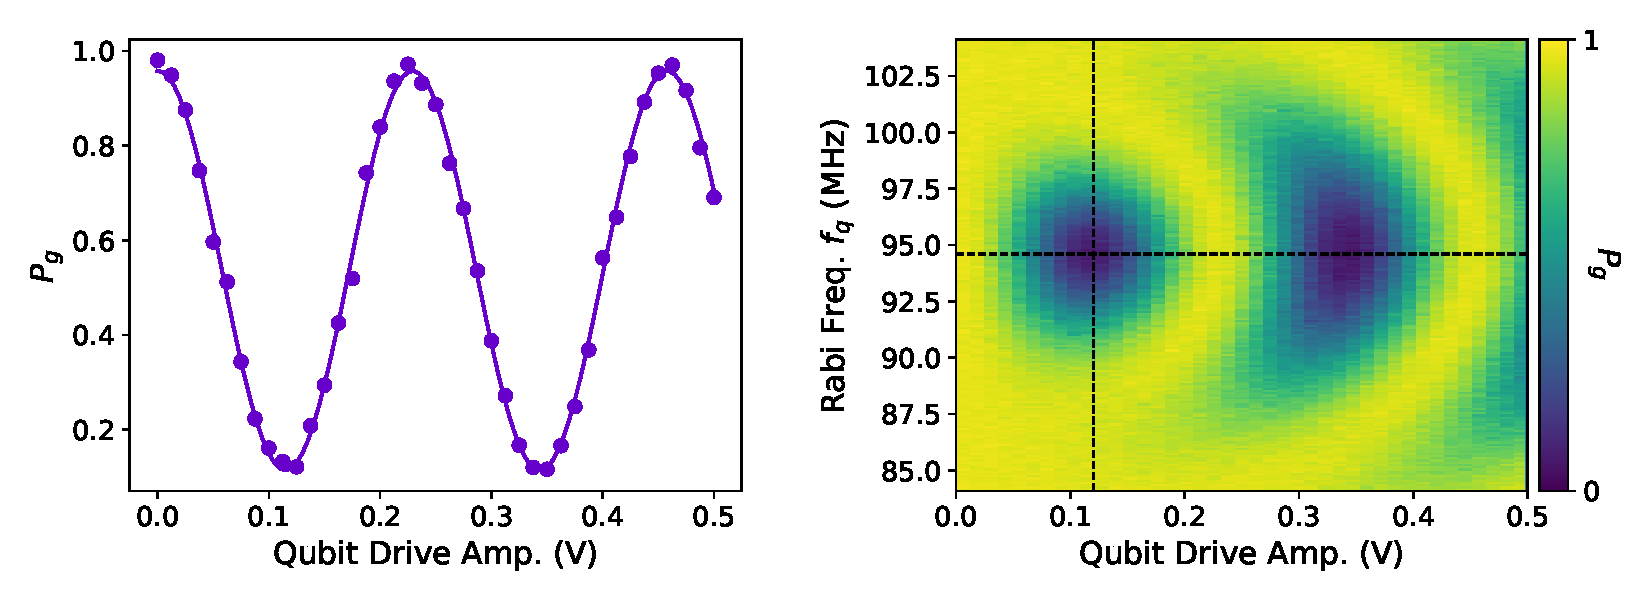
\includegraphics[width=0.95\linewidth]{Figures/4/rabi.pdf}
    \caption[Power Rabi experiment and Rabi chevrons.]{Left: Power Rabi experiment showing characteristic Rabi oscillations as we sweep the qubit drive amplitude for a resonant pulse. Right: we can sweep the frequency to get a ``chevron'' plot, and then use the minimum contrast point to tune up a $\pi$-pulse.}
    \label{fig:4_rabi}
\end{figure}

In subsequent measurements, we typically tuned up two kinds of $\pi$-pulses: the first was a shorter $\tau = 48$ ns pulse, which we used in most of the time-resolved qubit experiments. The second was a ``selective'' qubit pulse, of length $\tau = 2.4$ $\mu$s, chosen so that the associated spectral bandwidth of the pulse $1/\tau$ was smaller (at least at half-flux) than the dispersive shift $\chi$ between the qubit and storage mode (cf. Sec \ref{sec:4_StorageChi} where we discuss this further). We also later switched from Gaussian to cosine pulses; the latter were easier to work with due to their well-defined end points (zero amplitude at the start and end of the pulse). 

\subsection{Measuring the Fluxonium \texorpdfstring{$T_1$}{T1}\label{sec:4_fluxonium_T1}}

Our next set of experiments involved measuring the $T_1$ relaxation time of the fluxonium. The post-selection sequence we used to realize the measurement consists of two readouts separated by a variable length delay. The first readout initializes the qubit in either $\ket{g}$ or $\ket{e}$, while the second is used to track a change of state. The result is a characteristic $T_1$ relaxation curve showing an exponential decay of the qubit populations with time. We show an example of such a curve in Fig. \ref{fig:4_qubit_T1_vs_flux_single}(a), from which we extract a decay constant $T_1 = 220 \pm 10$ $\mu$s. Panel (b) shows the results of the same experiment now repeated across various external flux biases: we see that the flux-dependence of the qubit $T_1$ is very sharply peaked and symmetric about half-flux, with a maximum value of $T_1 \approx 265$ $\mu$s.

\begin{figure}[h]
    \centering
    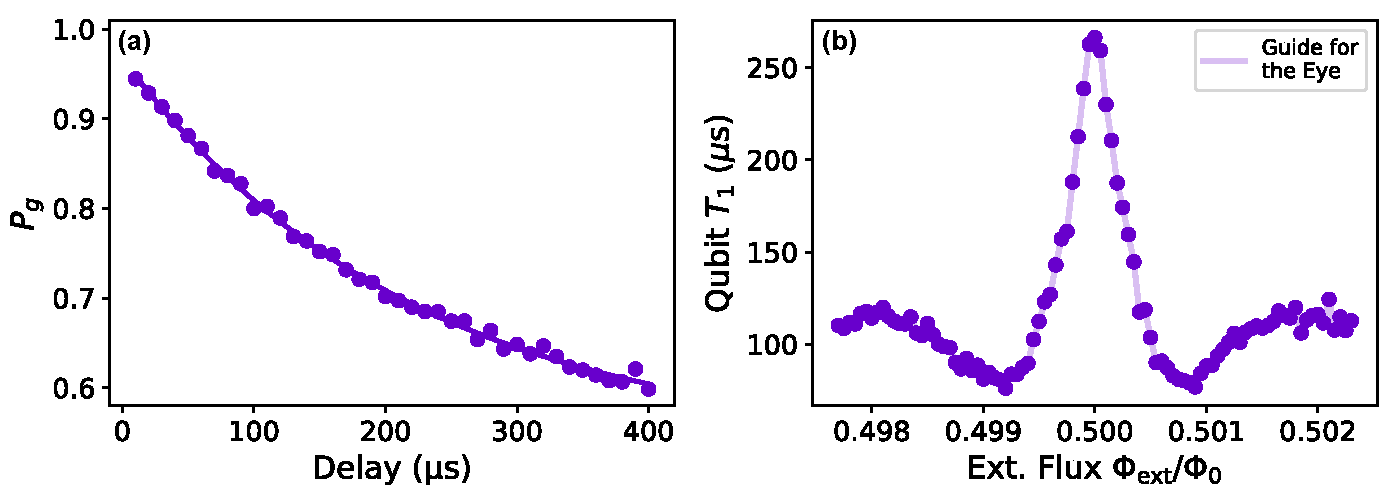
\includegraphics[width=0.95\linewidth]{Figures/4/qubit_T1_vs_flux_single.pdf}
    \caption[Qubit \texorpdfstring{$T_1$}{T1} experiment and sweep of \texorpdfstring{$T_1$}{T1} vs. flux.]{\textbf{(a)} $T_1$ experiment measuring qubit population $P_g$ vs. time. Solid line shows a fit to an exponential decay with an extracted $T_1 = 220 \pm 10$ $\mu$s. \textbf{(b)} Sweep of $T_1$ experiments vs. flux; at each flux, we tune up a $\pi$-pulse and then measure the $T_1$ decay.}
    \label{fig:4_qubit_T1_vs_flux_single}
\end{figure}

The sharply peaked flux-dependence in Panel \ref{fig:4_qubit_T1_vs_flux_single}(b) was one of the first experimental mysteries that we encountered with this device. For the parameters of our fluxonium, and assuming a capacitive (i.e., dielectric) loss model, we naively expected $T_1$ to improve away from half-flux. There are other loss models that would predict $T_1$ degrading away from half-flux (e.g., quasiparticle tunneling); however, we were unable to reproduce the sharp initial drop-off in any numerical simulations at the time of the experiment. [As we discuss below, however, we have since come up with a model that we believe may explain these observations]. 

If we go out even further in flux, we see an even richer structure to the flux-dependence of the fluxonium $T_1$ [see Fig. \ref{fig:4_qubit_T1_vs_flux_spec}]. Away from half-flux, we see a clear drop in $T_1$, followed by an apparent revival around $\Phi_{\rm ext} \approx 0.485\Phi_0$. However, as we move leftwards, we again see further drop-offs in the $T_1$. Although these observations puzzled us for some time, we eventually came to the hypothesis that the drop-offs in $T_1$ may be a form of Purcell decay.

\begin{figure}[h]
    \centering
    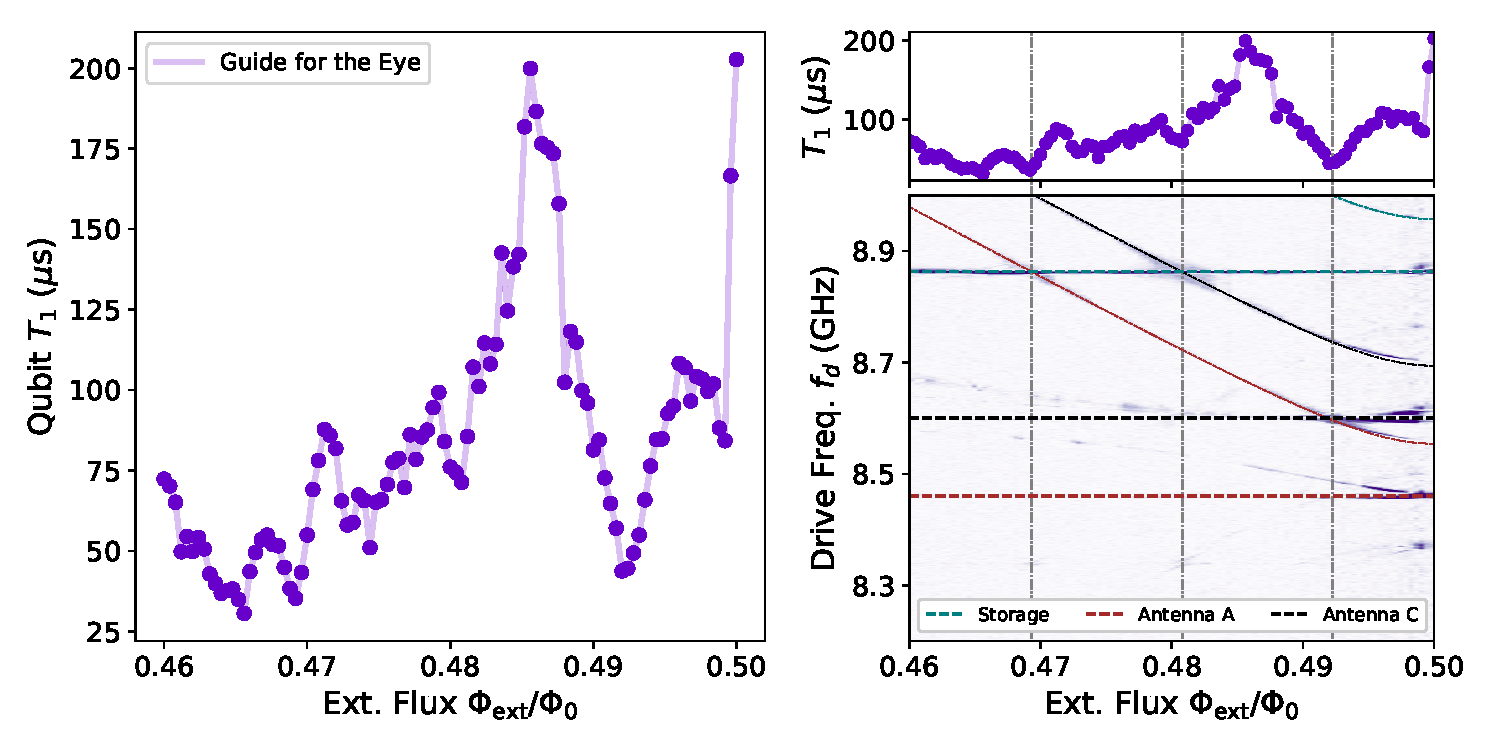
\includegraphics[width=0.95\linewidth]{Figures/4/qubit_T1_vs_flux_spec.pdf}
    \caption[Wider range sweep of qubit \texorpdfstring{$T_1$}{T1} vs. flux.]{Left: Sweep of $T_1$ experiment vs. flux over a wider range of external fluxes. We see rich structure, which we associate with accidential two-photon resonances in the spectrum. Right: we match the locations of the largest qubit $T_1$ drops to two-tone spectroscopy, showing that they coincide with the resonances shown. See main text for details.}
    \label{fig:4_qubit_T1_vs_flux_spec}
\end{figure}

In the right panel of Fig. \ref{fig:4_qubit_T1_vs_flux_spec}, we reproduce the $T_1$ data from the left panel, but also now align it with two-tone spectroscopy data taken earlier. At this resolution, the storage and the two antenna modes are straight lines. On top of these we see certain flux-dependent transitions: it turns out that these are ``two-photon'' transitions! (We showed these in Fig. \ref{fig:4_two_tone_vs_flux_full} as well). Specifically, they correspond to the frequencies of the linear modes \textit{plus} the qubit $\ket{g}\to\ket{e}$ frequency, i.e., they are activated when $\omega_d \approx \omega_{\rm lin} + \omega_{ge}$ where $\omega_{\rm lin}$ can be the frequency of the storage or either antenna. Intuitively, we can understand the drop-offs in qubit $T_1$ occurring when this ``two-photon'' transition is tuned into resonance with one of the \textit{other} linear modes. For example, at $\Phi_{\rm ext} \approx 0.48\Phi_0$, we have $\omega_{\rm C} + \omega_{ge} \approx \omega_{s}$, and at $\Phi_{\rm ext} \approx 0.47\Phi_0$, we have $\omega_{\rm A} + \omega_{ge} \approx \omega_{s}$. In both cases, the resulting resonance leads to a direct Purcell-type decay of the qubit. We have since been able to reproduce this behavior using numerical Purcell simulations, including the initial drop-off at half-flux shown in Fig. \ref{fig:4_qubit_T1_vs_flux_single}; although the latter does not correspond to a direct resonance, we suspect it arises as a higher order term in perturbation theory. I will leave a full investigation of this effect to future work. 

\subsection{Ramsey and Echo Measurements}

We also performed coherence measurements of the qubit using typical $T_2$ Ramsey and Echo sequences. A Ramsey measurement involves applying two ($\pi/2$)-pulses separated by a variable length delay $\tau$; by detuning the frequency of the pulses from the actual qubit frequency, we observe characteristic Ramsey oscillation fringes of the qubit population vs. time with a frequency given by the detuning \cite{raimond2006exploring, krantz2019quantum, naghiloo2019introduction}. An Echo measurement is similar, but adds an additional $\pi$-pulse in the middle of the sequence to refocus dephasing errors; in this case, all pulses are set to be resonant with the qubit and we see no oscillations. In both cases, the overall envelope decays with time and we can fit this decay to the function $A\cdot\exp[-(\tau/T_2)^{1 +\alpha}]$, where $A$ is an overall amplitude, $T_2$ is the characteristic \textit{coherence} time, and $\alpha$ is a parameter that depends on the noise statistics\footnote{When $\alpha = 0$, we get an overall exponential decay characteristic of white noise. Meanwhile $\alpha=1$ results in a Gaussian decay, which is characteristic of $1/f$ flux noise.} with typical values between 0-1 \cite{ithier2005decoherence, hutchings2017tunable, didier2019ac}. We can further separate $1/T_2 = 1/2T_1 + 1/T_\varphi$, where $T_1$ is the relaxation time from before and $T_\varphi$ corresponds to the pure dephasing time \cite{krantz2019quantum}. In our device, we had $T_1 \gg T_2$, and thus $T_\varphi \approx T_2$. We show typical Ramsey and Echo  measurements of our fluxonium in Fig. \ref{fig:4_T2_ramsey_echo}, taken with the qubit parked at the half-flux sweet spot. 
\begin{figure}[h]
    \centering
    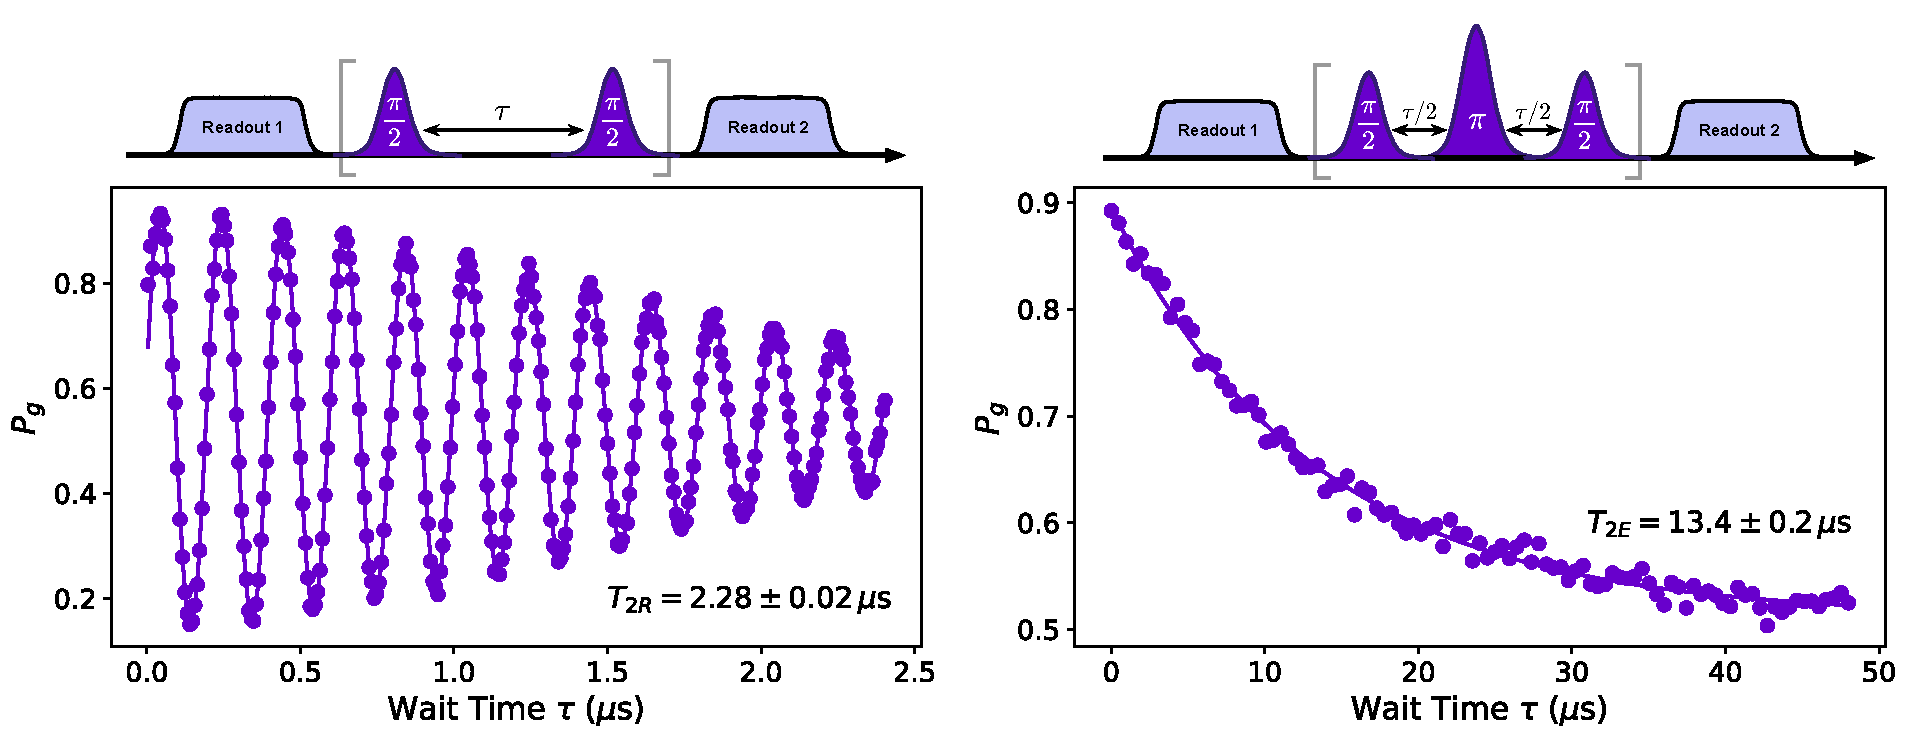
\includegraphics[width=0.95\linewidth]{Figures/4/T2_ramsey_echo.pdf}
    \caption[Qubit \texorpdfstring{$T_2$}{T2} Ramsey and Echo measurements.]{$T_2$ measurements for our fluxonium at half-flux. \textbf{(a)} The Ramsey experiment reveals $T_{2R} = 2.28 \pm 0.02$ $\mu$s. Oscillation fringes were introduced by detuning the qubit pulses from the qubit frequency. \textbf{(b)} The Echo measurement reveals $T_{2E} = 13.4 \pm 0.2$ $\mu$s. }
    \label{fig:4_T2_ramsey_echo}
\end{figure}

% \todo{Perhaps mention flux noise amplitude if there is space for it.}

\clearpage
\section{Storage Resonator Measurements \label{sec:4_StorageChi}}

\subsection{Storage Spectroscopy}

We are now ready to discuss measurements of the storage resonator. At this stage, we had already identified the storage in two-tone spectroscopy, and now wanted to corroborate this using a storage spectroscopy experiment. This measurement uses the qubit as a meter to probe the storage resonator frequency; as shown below in Fig. \ref{fig:4_storage_spectroscopy}, it involves driving the storage resonator and then performing a frequency-selective $\pi$-pulse on the qubit. This $\pi$-pulse is chosen to have length $\tau \gg 1/\chi_{qs}$ and a frequency that corresponds to the qubit frequency when the storage has zero photons. When the initial storage drive is resonant with the cavity, it will displace the storage away from the vacuum $\ket{0}$; as a result, the $\pi$ pulse fails. Only when the storage drive is off-resonant will the cavity remain in its $\ket{n=0}$ state, and thus cause the $\pi$-pulse to be implemented correctly. Finally, given our need for post-selection here, we can initialize the fluxonium in either $\ket{g}$ or $\ket{e}$ to see two different resonance dips. In practice, we used a constant $\tau = 2.4$ $\mu$s for the selective pulse.
\begin{figure}[h]
    \centering
    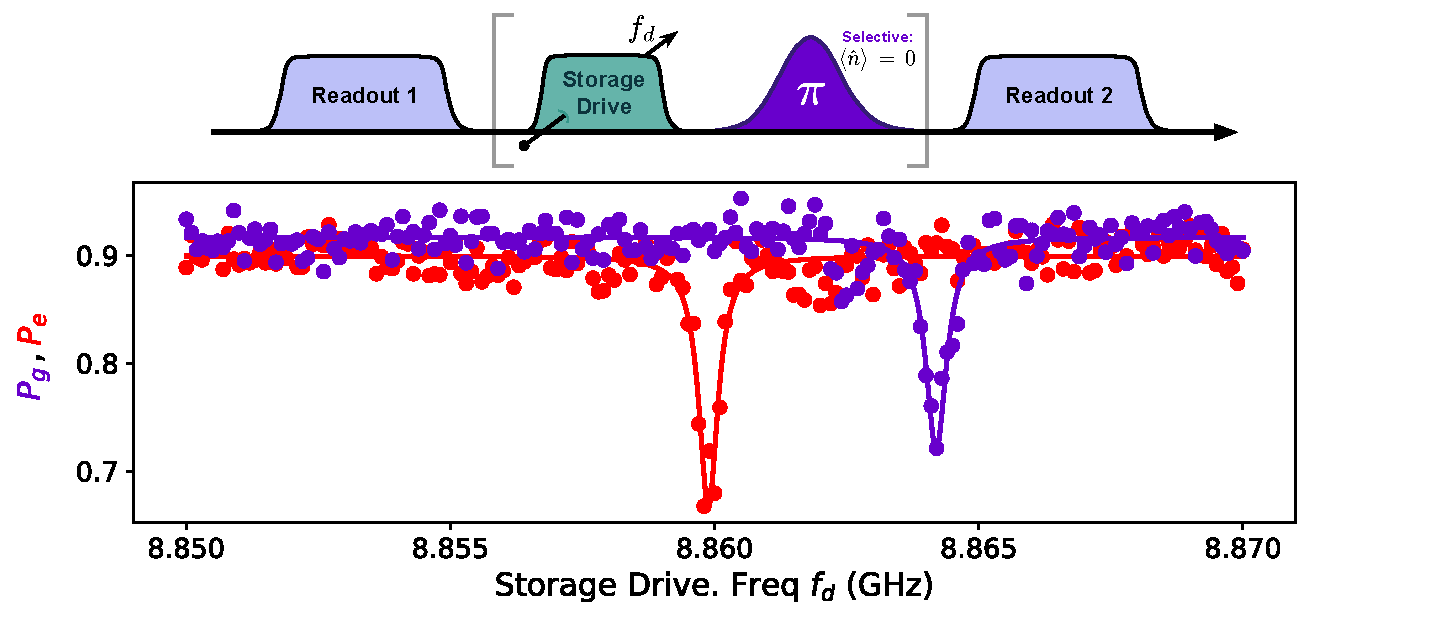
\includegraphics[width=0.85\linewidth]{Figures/4/storage_spectroscopy.pdf}
    \caption[Storage spectroscopy measurement.]{Storage spectroscopy measurement via the qubit. This experiment enables us to determine the storage frequency when the qubit is in $\ket{g}$ or $\ket{e}$ respectively.}
    \label{fig:4_storage_spectroscopy}
\end{figure}

\subsection{Engineering a Tunable Dispersive Shift}

The storage spectroscopy measurement above presents a method to extract the dispersive shift $\chi_{qs}$ between the fluxonium and storage. We simply sweep the external flux $\Phi_{\rm ext}$ and tune up a frequency-selective $\pi$-pulse at each bias point. Since the storage flux dispersion is minimal, we can perform a storage spectroscopy at each flux, and calculate $\chi_{qs}$ as the difference in the resonance frequency when the qubit is in $\ket{g}$ vs. $\ket{e}$, as is consistent with a Hamiltonian coupling term $\chi_{qs} \hat{a}^\dagger\hat{a}\sigmaz/2$. The result of this measurement is shown in Fig. \ref{fig:4_tunable_chi}, and we see that the dispersive shift indeed tunes with flux and crosses through zero, as is expected with bosonic mode threading. 

\begin{figure}[h]
    \centering
    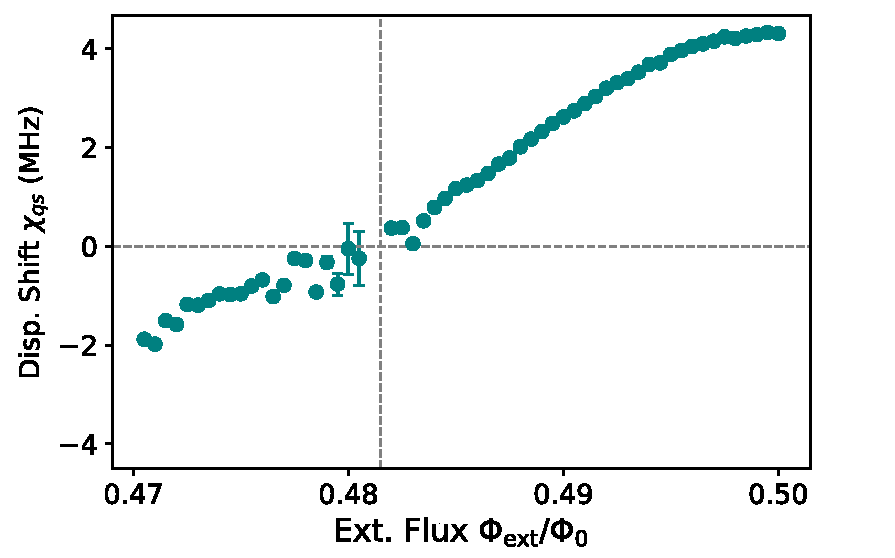
\includegraphics[width=0.6\linewidth]{Figures/4/tunable_chi.pdf}
    \caption[Demonstration of a flux-tunable storage dispersive shift.]{Measurement of the tunable storage dispersive shift $\chi_{qs}(\Phi_{\rm ext})$ vs. the external flux $\Phi_{\rm ext}$. We mark the approximate zero crossing point, which occurs at $\Phi_{\rm ext} \approx 0.481\Phi_0$.}
    \label{fig:4_tunable_chi}
\end{figure}

Given that we used a selective $\pi$-pulse of the same length $\tau = 2.4$ $\mu$s at each flux point, we do not expect this measurement technique to work well near the zero crossing point where $\chi_{qs} \to 0$, since there the condition $\tau \gg 1/\chi_{qs}$ ceases to hold. We consequently see slightly larger error bars at the crossing and cannot measure the exact point at which $\chi_{qs}=0$ (the fit fails there). 

\clearpage

\section{Storage Coherence: Problems and Pitfalls \label{sec:4_StorageCoherenceProblems}}

Our next experimental step was to characterize the coherence of the storage resonator. As we later discovered, however, the storage lifetime was severely limited in our device. This led to a series of A/B tests and many months of debugging before we realized that the problem was in some sense inherent to our design. In this section, we will present some of the major clues that led us to this conclusion. 

\subsection{Initial Time-Domain Measurement}

The first method we took to measure the storage lifetime was based on a number-splitting spectroscopy experiment \cite{schuster2007resolving}. This measurement sequence uses a selective qubit $\pi$-pulse, and in particular consists of playing a storage drive at one of the storage peaks (e.g. $\omega_s^{\ket{g}}$) and then performing qubit spectroscopy with the selective pulse. If we post-select to have started with the qubit in $\ket{g}$, then this will enable us to see multiple resonance peaks in the qubit spectrum corresponding to the photon number distribution in the cavity after it is excited via the storage pulse. We can see an example of this on the left plot in Fig. \ref{fig:4_storage_T1_numsplit} below, which shows the photon number distribution (teal) after driving the storage with a 10 $\mu$s pulse, followed by a 2.4 $\mu$s selective qubit $\pi$-pulse. The distribution is specified via the depth of the various resonance dips, and is expected to follow a Poisson distribution as the storage is driven to a coherent state. We contrast this with the case when the storage pulse is not played (grey), resulting in just a single qubit spectroscopy dip corresponding to the storage having $\ket{n=0}$ photons. 

In order to measure the storage $T_1$ this way, we can introduce a variable delay between the storage drive pulse and the qubit $\pi$-pulse. During this time, the storage will experience photon loss $\kappa_{1s}\mathcal{D}[\hat{a}]$ and thus the number distribution will decay back down towards the vacuum. We can measure this decay by parking at, say, the $\ket{n=0}$ dip and recording the change in contrast vs. time. For single-photon loss rate $\kappa_{1s}$, we expect an initial coherent state $\alpha_0$ to decay as $\alpha(t) = \alpha_0 e^{-\kappa_{1s}t/2}$, i.e., so that $\bar{n}(t) = |\alpha(t)|^2 =  \bar{n}_0 e^{-\kappa_{1s}t}$ with $\bar{n}_0 = |\alpha_0|^2$. We can fit the decay of the $\ket{n=0}$ qubit spectroscopy dip by weighting $\bar{n}(t)$ via the Poisson distribution evaluated at $n = 0$. This gives us a fit function $P_{g, 0}(t) = 1-a\cdot\exp[-\bar{n}_0 e^{-\kappa_{1s}t}]$ for the decay, where $a$ is a scale parameter to account for the partial contrast. From this, we can extract the lifetime $T_{1s} = 1/\kappa_{1s}$. We show the result of such a measurement in the right panel of Fig. \ref{fig:4_storage_T1_numsplit}.
\begin{figure}[h]
    \centering
    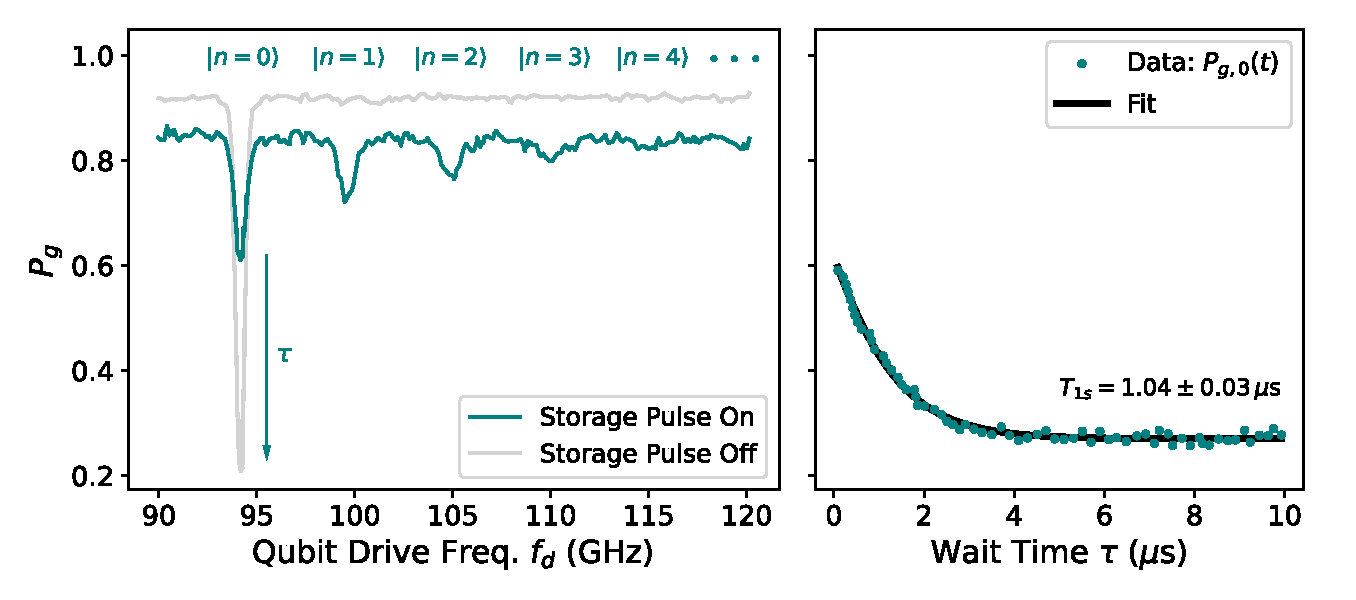
\includegraphics[width=\linewidth]{Figures/4/storage_T1_numsplit.pdf}
    \caption[Qubit spectroscopy in the photon-number resolved regime and time-domain measurement of the storage resonator \texorpdfstring{$T_1$}{T1} lifetime.]{Left: Number-splitting spectroscopy data for the qubit at half-flux, showing multiple photon-resolved dips (teal) after driving the storage for 10 $\mu$s. If we add a variable delay after the storage pulse, we observe the number distribution decaying back towards the case when the storage has $\ket{n=0}$ photons (grey). Plotting the depth of the $\ket{n=0}$ dip vs. time allows us to measure the single-photon decay and extract the storage lifetime.}
    \label{fig:4_storage_T1_numsplit}
\end{figure}

\subsection{Testing and Progress}
We were very surprised to measure a storage lifetime of $T_{1s} \approx 1$ $\mu$s, given the bare lifetime of the Mark II storage cavity of $T_{1s}^{\rm bare} \approx 765$ $\mu$s that we had seen previously without qubit chips. We therefore set out to debug this part of our system over several subsequent cooldowns. In time, we were able to verify that our bare 3D cavity resonators indeed had high coherence; we tested both the Mark II and Mark III cavities in various configurations as shown in Fig. \ref{fig:4_3D_Cavity_Debugging}. These tests also helped us rule out excess coupling loss due to the storage drive pin. One observation we made is that even inserting blank Si chips (i.e., with no qubit, flux line, or metallization) into the cavities seemed to degrade their lifetime from above 1 ms to approximately 100 $\mu$s. We attributed this to lossy backside of the qubit chip, since the Si wafer used to fabricate the fluxonium devices was only single-side polished\footnote{This was an aberration in the fabrication process used for our devices, since the 8" Si process was still being developed at that time. One should otherwise always use a double-side polished wafer since the backside of the chip can also introduce unwanted dielectric losses!}. Nonetheless, this effect alone was not enough to account for the drop in cavity coherence from over 760 $\mu$s to $\sim\!1$ $\mu$s. 

\begin{figure}[t]
    \centering
    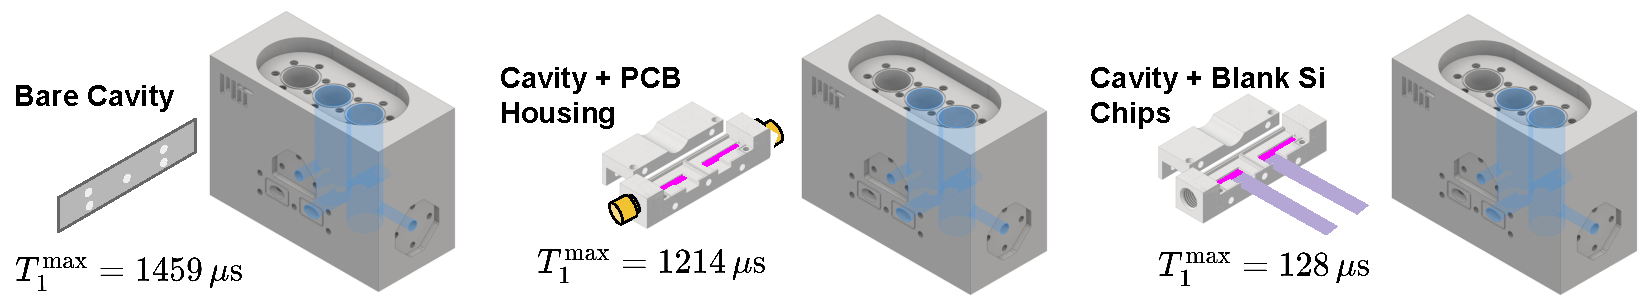
\includegraphics[width=\linewidth]{Figures/4/3D_Cavity_Debugging.pdf}
    \caption[Attempts to debug low storage lifetime in different configurations.]{Maximum single-photon $T_{1s}$ measured across all three resonators of the Mark III cavity. We calculate $T_{1s}$ using a frequency-domain measurement of the cavity using a Vector Network Analyzer. Each configuration was tested during a different cooldown of the fridge.}
    \label{fig:4_3D_Cavity_Debugging}
\end{figure}

Our main suspicion was that the storage loss was coming primarily from the qubit flux line; we thus first attempted to remedy it by adding external DC/RF filtering to our lines. Unfortunately, this is did not seem to solve the problem. We later also attempted capping the flux line with a 50 $\Omega$ terminator and then went as far as fully de-wirebonding it; neither of these changes helped appreciably and the storage lifetime remained around 1 $\mu$s or less. Our conclusions from these tests were also muddied by uncontrolled factors between the various cooldowns (e.g., statistical variations in lifetime, degradation of the cavities with time, or changes to the exact amount of indium used in the seals). 

\subsection{Direct Measurement of Loss from the Flux Line}

We were ultimately able to confirm our suspicions about the flux line loss by performing a direct reflection ($S_{11}$) measurement of the 3D cavities \textit{through} the flux lines. We connected a VNA to the flux line and were able to measure the storage cavity resonance, which alone was enough to tell us that the flux line was too strongly coupled (cf. Fig. \ref{fig:4_storage_loss_thru_flux_line}); we ideally should not be able to see anything. Here, however, the low-power resonator spectroscopy measurement shows two dips associated with the qubit being in $\ket{g}$ or $\ket{e}$ respectively (since we had the flux line connected and biased near half-flux). To reflect this, we fitted the data to a double Lorentzian $S_{11}$ model consisting of two weighted peaks with identical linewidths but different frequencies. From here, we were able to extract $\kappa_c/2\pi = 320.9$ kHz and $\kappa_i/2\pi = 2.03$ MHz. 

\begin{figure}[h]
    \centering
    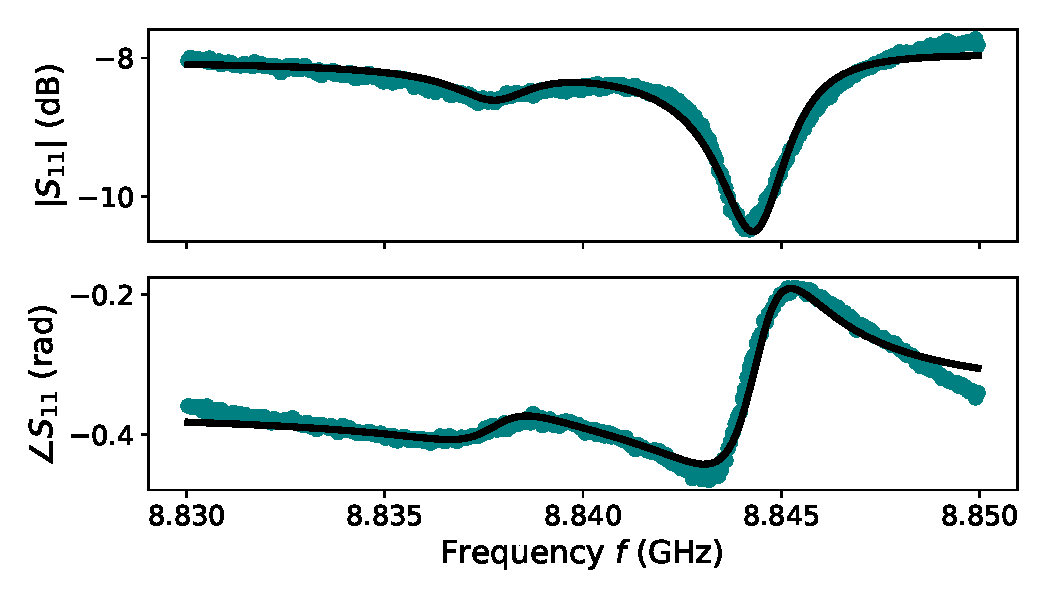
\includegraphics[width=0.7\linewidth]{Figures/4/storage_loss_thru_flux_line.pdf}
    \caption[Direct measurement of the storage resonator through the qubit flux line.]{Direct measurement of the storage resonance through the qubit flux line. At half-flux, we see two peaks associated with the states $\ket{g}$ and $\ket{e}$. We fit data to a double Lorentzian $S_{11}$ model with two weighted peaks of identical linewidth to extract $\kappa_c$ and $\kappa_i$.}
    \label{fig:4_storage_loss_thru_flux_line}
\end{figure}

In the configuration of measuring $S_{11}$ through the flux line, the constant $\kappa_c$ tells us how much of the total storage loss comes from its coupling to the flux line. We get $T_{1c} = 1/\kappa_c \simeq 0.496$ $\mu$s, thus confirming that the flux line is limiting. However, in this measurement, we found that the internal loss $\kappa_i$ is even larger than $\kappa_c$, suggesting there is \textit{another} loss channel at play beyond just the flux line. 

\subsection{Storage Loss HFSS Simulations and Summary}

We were finally able to resolve the storage loss question by revisiting our E\&M eigenmode simulations of the 3D cavity package using Ansys-HFSS\footnote{I'd like to thank R\'eouven Assouly for his insight to re-run the simulations, for various tips for using HFSS, and his help and willingness to brainstorm creative solutions during this turbulent time in the project.}. We found that the storage losses were significant even in simulation and thus inherent to our design. This is ultimately the reason why many of the steps we took during our A/B testing did not improve the cavity lifetimes. We show an example simulation in Fig. \ref{fig:4_HFSS_Simulation}, here characterizing the effect of 50 $\Omega$ loss from the flux line [panel (a)]. We consistently found that when the fluxonium chip is inserted, the electric field of the storage mode does \textit{not} stay confined to the post cavity, but instead `leaks out' and does so in two distinct ways: (i) through the qubit flux line, as shown in panel (d), and (ii) by participating in the ground plane mode between the chip and the tunnel walls, as shown in panel (e). We found in simulation that the former effect (i) seemed to depend significantly on the shape of the flux line tip. In particular, using an exact model of the flux line [Fig. \ref{fig:4_HFSS_Simulation}(b)] resulted in a storage lifetime of $T_{1s} \simeq 0.5$ $\mu$s in simulation, whereas using an approximate model [Fig. \ref{fig:4_HFSS_Simulation}(c)] gave a lifetime of $T_{1s} \simeq 1.9$ ms --- roughly four orders of magnitude higher! This discrepancy is likely the reason why we did not catch this error during the initial design/simulation of the 3D cavity system; in turn, this resulted in significant storage loss down the flux line that we saw in experiment and showed in Fig. \ref{fig:4_storage_loss_thru_flux_line}.

\begin{figure}[t]
    \centering
    \includegraphics[width=0.8\linewidth]{Figures/4/HFSS_Simulation.pdf}
    \caption[HFSS electromagnetic simulations of the 3D cavity-fluxonium architecture showing storage losses inherent to the design.]{\textbf{(a)} HFSS model of our 3D cavity-fluxonium device with a 50 $\Omega$ loss channel. \textbf{(b, c)} Exact and approximate models for the tip of the flux line. \textbf{(d)} Eigenmode simulation result showing storage cavity electric field; the field is mostly concentrated around the post cavity, but also leaks down the flux line. \textbf{(e)} Different angle showing the cavity field also participating in the ``ground plane'' mode, and thus leading down the chip tunnel.}
    \label{fig:4_HFSS_Simulation}
\end{figure}

As the experimental data also suggested, however, the latter source of loss due to storage participation in the ground plane mode was also significant, and thus something we tried to reproduce in simulation. This effect (ii) is more subtle, and arises when a voltage develops between the ground plane metallization of the qubit chip and the tunnel wall of the 3D cavity, giving rise to a $(\lambda/4)$-like mode of the entire ground plane. The storage participates in this spurious mode and thus its field can be thought to `leak' down the tunnel. As a result, the storage will experience a full litany of loss mechanisms that 3D cavities are otherwise supposed to be resilient to by design (e.g., seam loss at the mouth of the tunnel and mode participation in lossy glue and/or PCB dielectrics) \cite{reagor2013reaching,brecht2015demonstration,reagor2016quantum}. We corroborated this in simulation by later including seam loss explicitly. From these simulations, we realized that the ``ground plane'' loss channel (ii) will always arise if there is significant metallization inside the chip tunnel. While this could in principle be alleviated by somehow grounding the chip to the 3D cavity tunnel walls (e.g., using indium), doing so would necessarily also introduce seam losses, and thus it is not immediately clear how to proceed. Meanwhile, the ``flux line'' loss (i) could be solved in several ways, such as by using some form of on-chip microwave filtering \cite{pozar2012microwave} (more discussion of this in Ch. \ref{ch:5_2DGKP}).  

In summary, we learned from our experiments that it is a difficult technical challenge to integrate a fast-flux line in 3D while maintaining the coherence of an otherwise high-Q cavity. Although this presents a major hurdle for using fluxonium in a 3D-cavity architecture for the purpose of bosonic QEC, there are potential paths forward. We will discuss a few such approaches in the upcoming chapter. 

\clearpage
\printbibliography[heading=subbibliography, title = References]